\documentclass{beamer}
\usetheme{CENIDETDIE}
\setbeamertemplate{caption}[numbered]
\usefonttheme[onlymath]{serif}

% ------------------------------------------------------------------------------------------------

\usepackage[utf8]{inputenc}
\usepackage[T1]{fontenc}
\usepackage{helvet}
\usepackage{graphicx} % Allows including images
\usepackage{booktabs} % Allows the use of \toprule, \midrule and \bottomrule tables
\usepackage{amsmath} % Allows the use of $...\text{normal text}...$
\usepackage{color}
\usepackage{hyperref}
%\usepackage{showframe}
\usepackage[absolute,overlay]{textpos} %To place the images
\usepackage[document]{ragged2e}
%\usepackage{authblk} %many authors
%\numberwithin{figure}{section}
%\usepackage{ragged2e}%To use justify
%\numberwithin{equation}{section}
%\usepackage{natbib}
\usepackage{multirow}
%\usepackage{apalike}
\usepackage{biblatex}
\addbibresource{references.bib}
%\usepackage[bottom]{footmisc}
%\usepackage[colorinlistoftodos]{todonotes}
\usepackage{graphicx}
\usepackage{caption}
\usepackage{subcaption}
\usepackage{setspace}
%\usepackage{setspace}
%\renewcommand{\baselinestretch}{1.0} 
% ------------------------------------------------------------------------------------------------
\title{\textbf{ \textit{Simplest Fermion Vector-Like Portal Dark Matter model:}}}
\subtitle{{\small 	Search in the compressed mass region at the CMS experiment}}
\author[C.Salazar]{\textbf{Camilo Salazar} }
\institute[UdeA]{camilo.salazar@cern.ch}

%\author{\textit{\textbf{Camilo A Salazar G}}}
%\institute{\url{camilo.salazar@cern.ch} }
\date{\today}


% ------------------------------------------------------------------------------------------------

\begin{document}

% ------------------------------------------------------------------------------------------------

\begin{frame}[plain,t]
\titlepage
\end{frame}


% ------------------------------------------------------------------------------------------------

\begin{frame}[plain,noframenumbering]
  \addtocounter{framenumber}{-1}
  \scriptsize
%   \thispagestyle{empty}
  \frametitle{Contenido}
  \setbeamertemplate{section in toc}[sections numbered]
  \tableofcontents[hideallsubsections]
\end{frame}

% ------------------------------------------------------------------------------------------------

\section{Introduction}
\begin{frame}
\frametitle{Introduction}
\justifying{
	

Dark Matter (DM) constitutes one of the main unsolved problems in fundamental physics. 
Ever since it was proposed to explain the rotation curves of galaxies, 
some other astronomical observations left little doubt of its existence.
\vspace{5 mm}

Whatever DM is, the Standard Model (SM) is not able to produce a candidate that has, at present in the universe, stability and also interact very little or not at all with the known matter, proven properties of DM. 

}


\end{frame}

% ------------------------------------------------------------------------------------------------

\begin{frame}
\frametitle{Rotational Velocities}


\begin{figure}[!tbp]
\centering
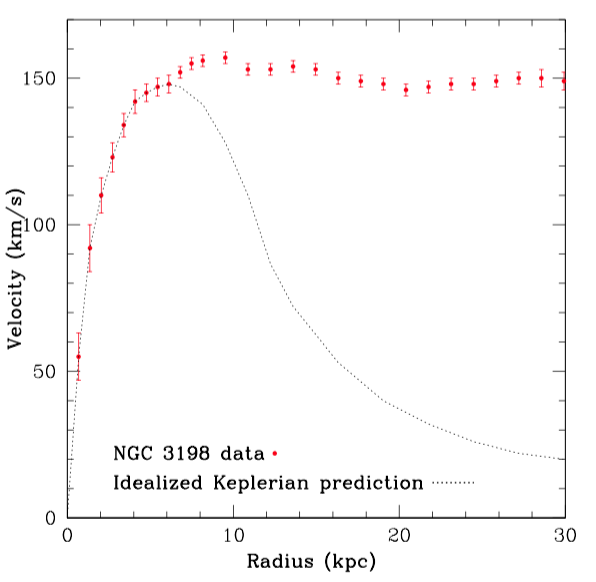
\includegraphics[width=0.6\textwidth]{pictures/fig_Introduction_rotation_curve_1}\label{fig:f1}
\caption{{\scriptsize Measured rotational velocities of HI regions in NGC 3198 compared to an idealized Keplerian behavior [Astron. and Astrophys. 223, 47-60]}}
\end{figure}

\end{frame}

% ------------------------------------------------------------------------------------------------

\begin{frame}
\frametitle{Bullet cluster}


\begin{figure}[!tbp]
\centering
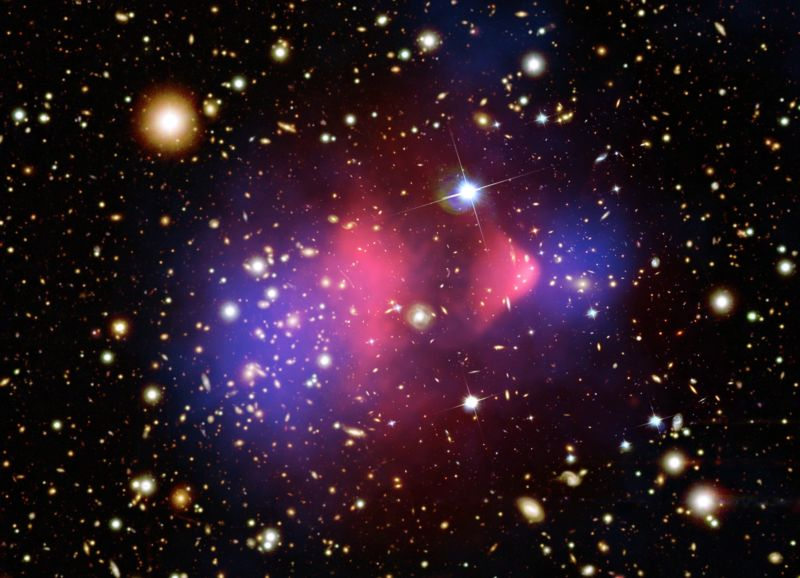
\includegraphics[width=0.8\textwidth]{pictures/bulletcluster}\label{fig:f2}
\caption{{\scriptsize The Bullet cluster, the result of a subcluster (the “bullet”) colliding with the larger galaxy cluster 1E 0657-56  [arXiv:1711.02117]}}
\end{figure}

\end{frame}

% ------------------------------------------------------------------------------------------------


\section{Motivation}
\begin{frame}
\frametitle{Motivation}

\begin{figure}[!tbp]
\centering
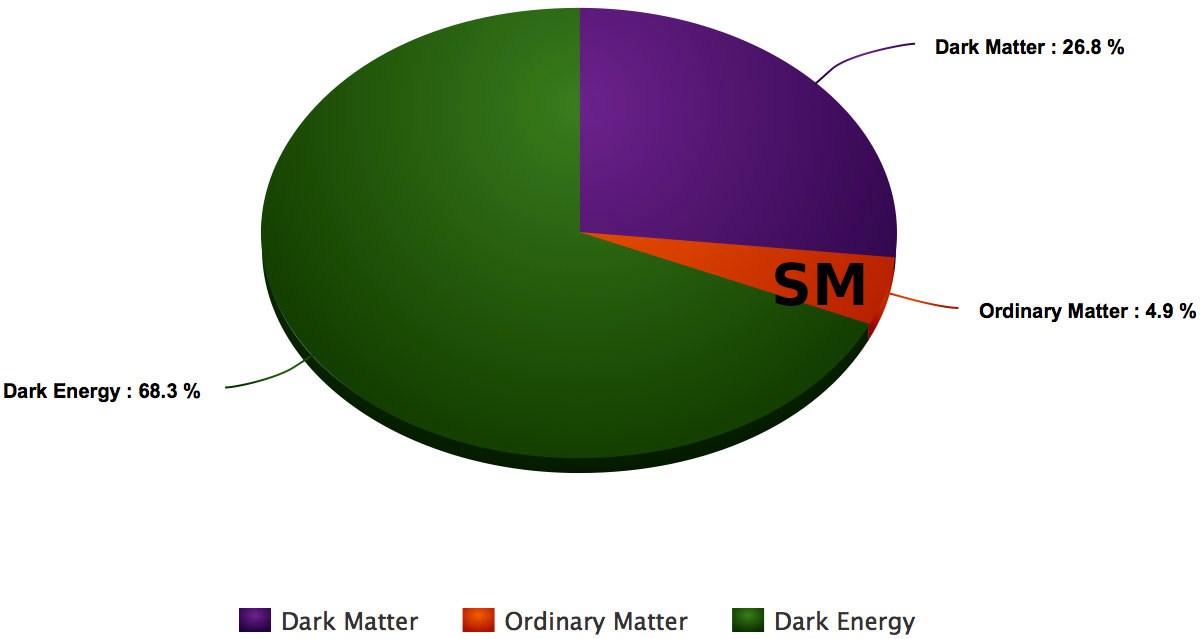
\includegraphics[width=0.9\textwidth]{pictures/pie.png}\label{fig3}
\caption{{\scriptsize Simplified plot showing the estimate abundances, of the known components of the universe. }}

\end{figure}

\end{frame}

% ------------------------------------------------------------------------------------------------

\begin{frame}
\frametitle{Detection Channels}

\begin{figure}[!tbp]
\centering
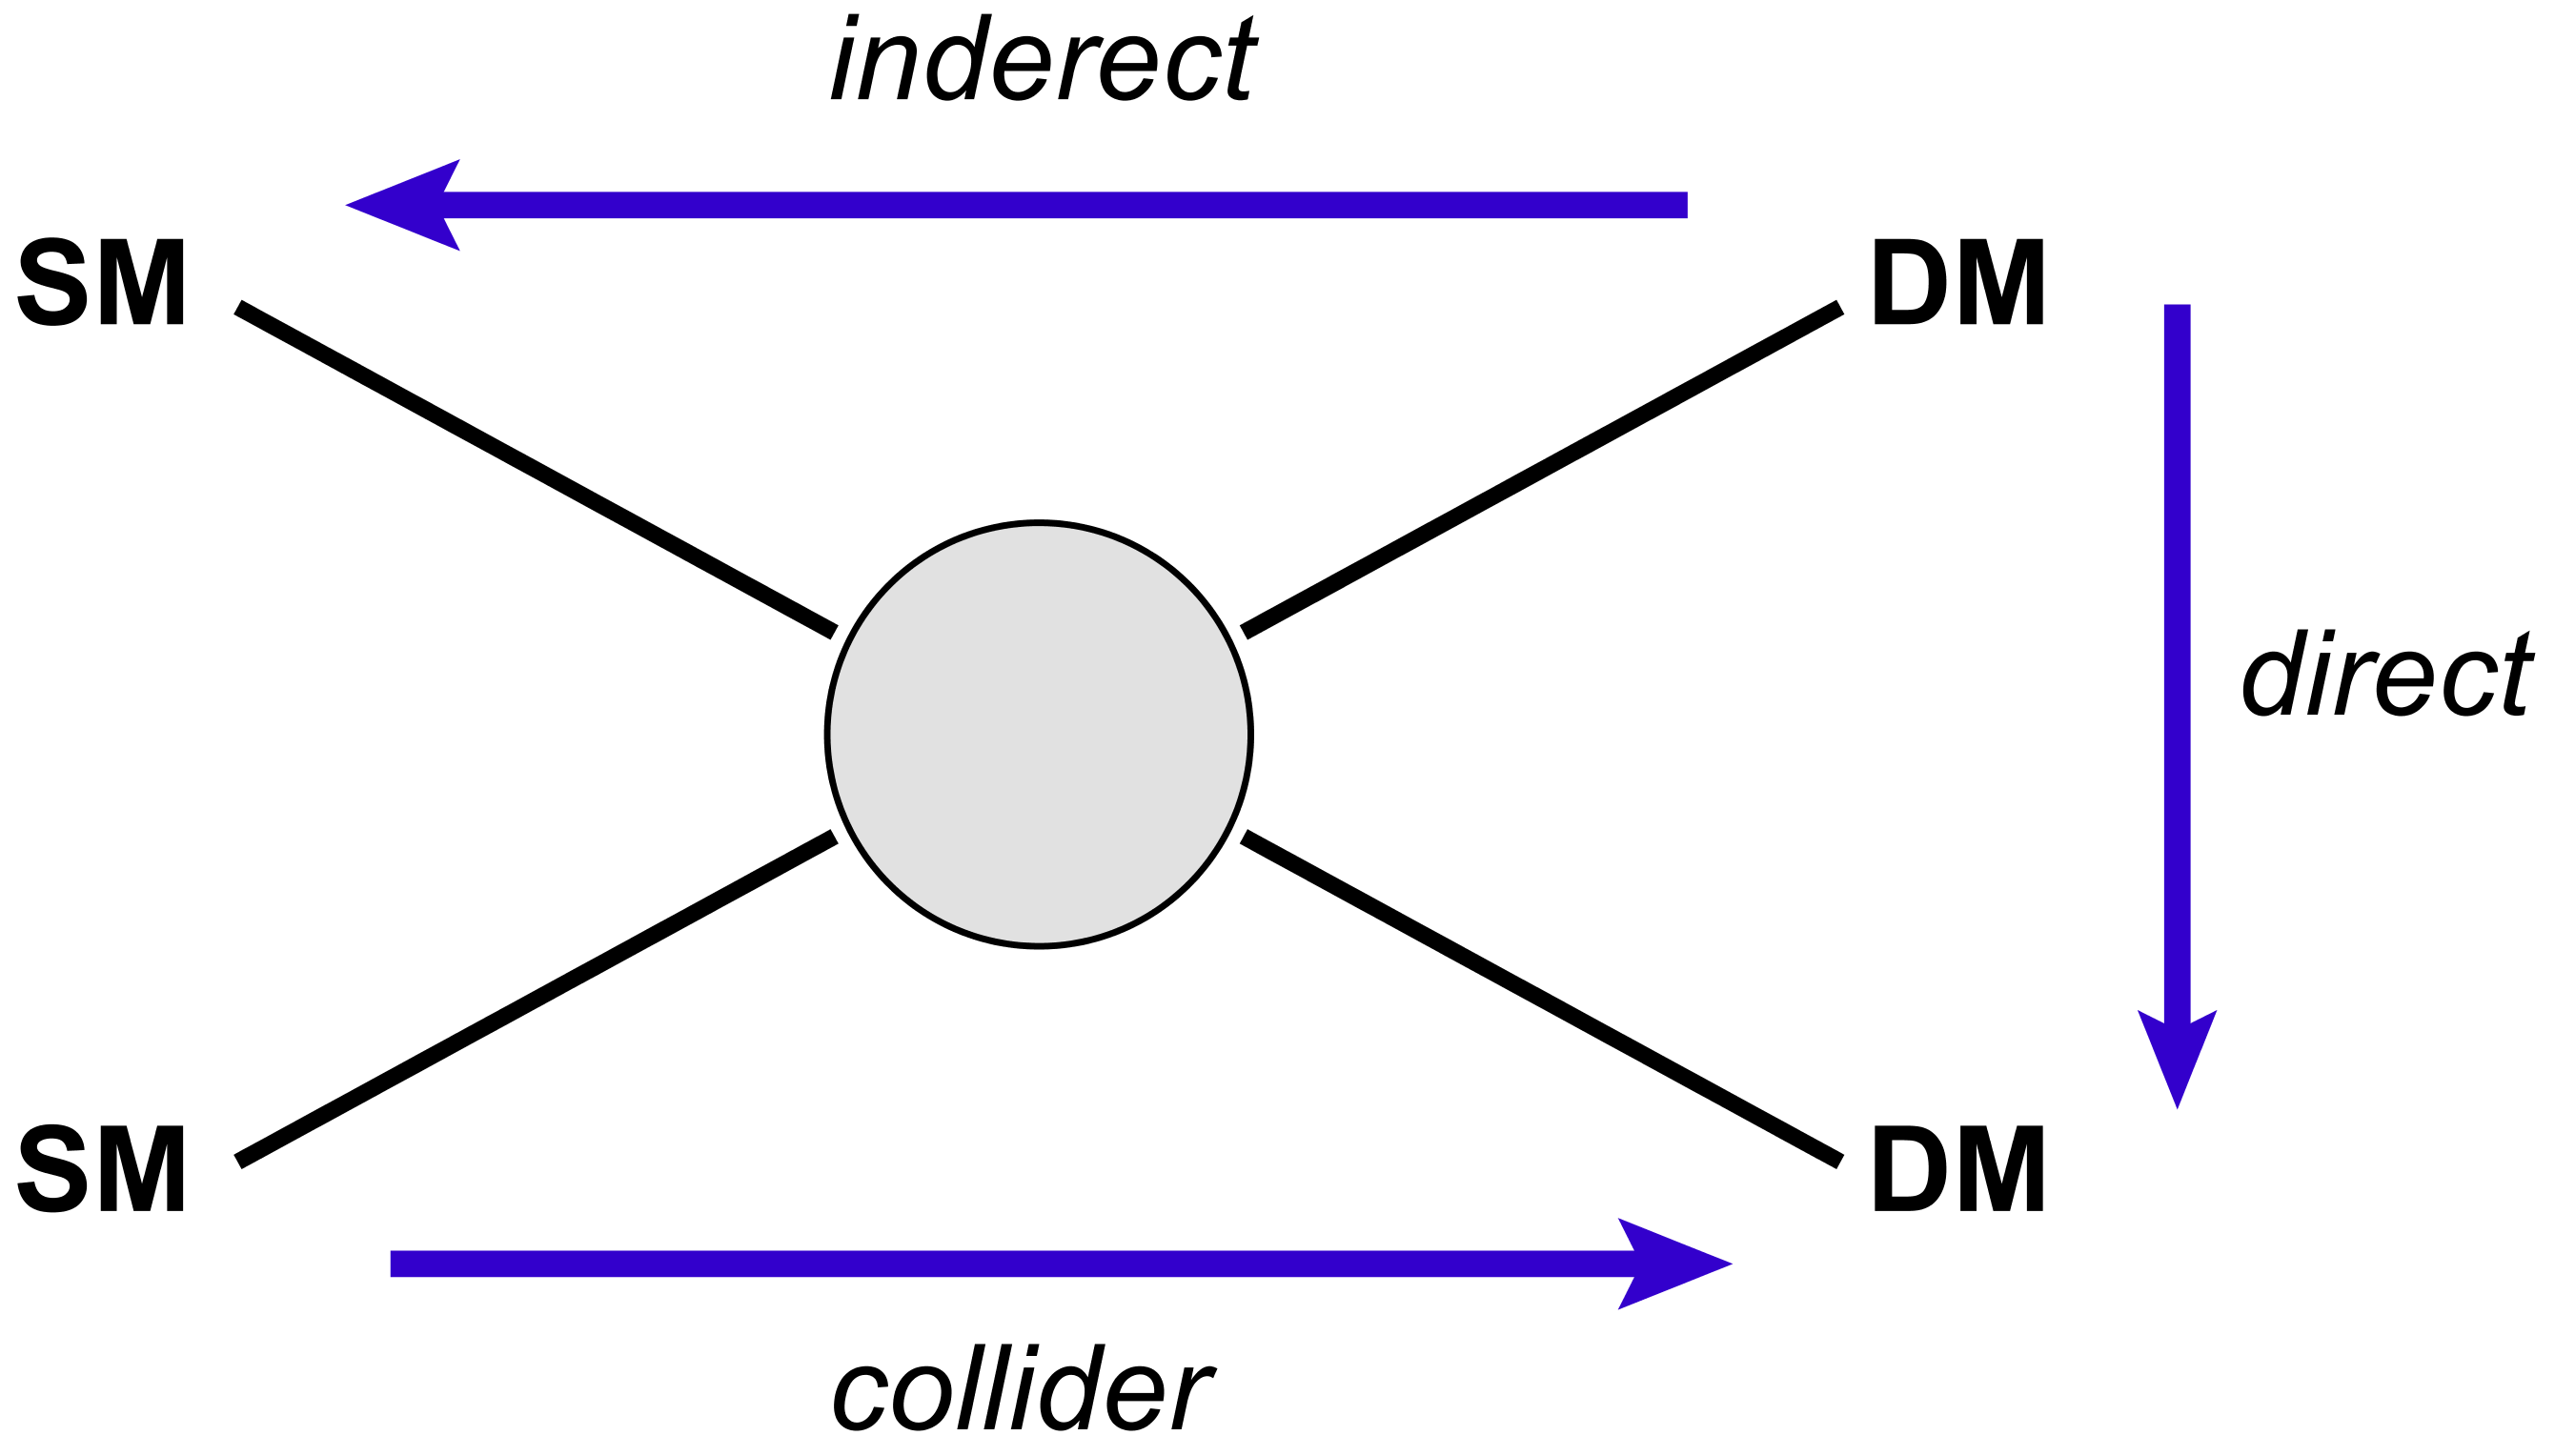
\includegraphics[width=0.9\textwidth]{pictures/Schem}\label{fig4}
\caption{{\scriptsize Schematic showing the possible dark matter detection channels.}}

\end{figure}

\end{frame}
% ------------------------------------------------------------------------------------------------

%\begin{frame}
%\frametitle{Collider Detection}

%\begin{alertblock}{Signals}
%\begin{enumerate}
%\item Cascades of heavier particles to the DM candidate and SM, as in (\subref{Cascade}).
%\item[]
%\item DM production in association with other SM particles,    like (\subref{DirectProduction}).
%\end{enumerate}
%\end{alertblock}

%begin{figure}[!h]

%\begin{subfigure}[b]{0.44\textwidth}
%\centering
%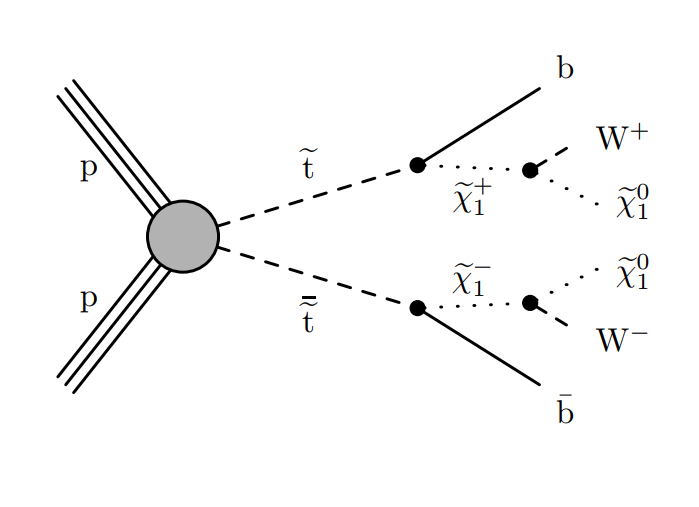
\includegraphics[width=\textwidth]{pictures/Cascade}
%\caption{}
%\label{Cascade}
%\end{subfigure}
%\begin{subfigure}[b]{0.44\textwidth}
%\centering
%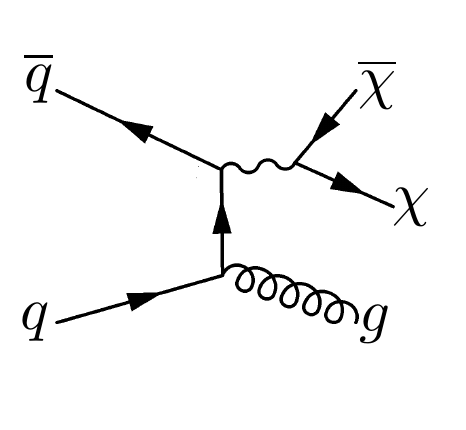
\includegraphics[scale=0.3]{pictures/DirectProduction}
%\caption{}
%\label{DirectProduction}
%\end{subfigure}

%\end{figure}



%\end{frame}
% -------------------------------------------------------------------------

% ------------------------------------------------------------------------------------------------

\section{Model}
\begin{frame}
\frametitle{Model}
\begin{justify}

The VLF model introduce a vector-like charged fermion with $SU(2)_L$ singlet, a scalar particle and a $Z2$ symmetry to guarantee the stability of the DM candidate. The free Lagrangian reads
\begin{equation}\nonumber
\mathcal{L} = \mathcal{L}_{SM} +  m_F \bar{F}F + ( Y_\ell S \bar{F}\ell_R + {\rm h.c.} ) + V(S,H)~;
\end{equation}\label{EQ}
$m_F$ is the singlet fermion mass parameter, $\ell_R$ are the SM right-handed lepton fields, $Y_\ell$ 
are the Yukawa couplings. The contribution to the scalar potential is given by
\begin{equation}\nonumber
V(S,H) = \frac{m_S^2}{2} S^2 + \frac{\lambda_S}{4} S^4 + \lambda_{SH} S^2|H|^2 ~,
\end{equation}
with scalar mass parameter $m_S$ and quartic couplings $\lambda_{S}$ and $\lambda_{SH}$.
\end{justify}

\begin{spacing}{0.5}
	{\tiny\textbf{Toma, T.} Internal bremsstrahlung signature of real scalar dark matter and consistency with thermal relic density. Phys. Rev. Lett. 111, (2013).}
	\vspace{4 mm}
\end{spacing}


\end{frame}
% ------------------------------------------------------------------------------------------------
% ------------------------------------------------------------------------------------------------
\begin{frame}
\frametitle{Kinetic Lagrangian}

\begin{textblock*}{0.5\linewidth}(0.75\linewidth,0.2\linewidth) % {block width} (coords)

\begin{figure}[!tbp]
\centering
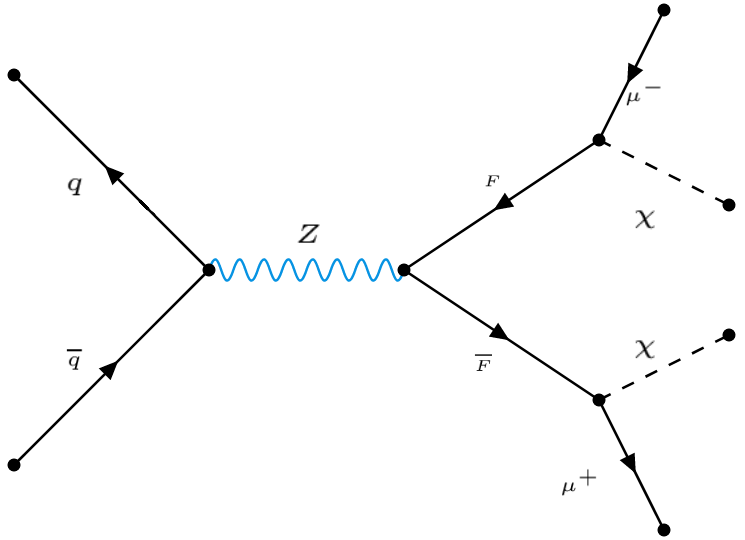
\includegraphics[width=1\textwidth]{pictures/DYVLFNoJet}
\caption{{\scriptsize Pair-production of vector-like fermions ($p p \to F^- F^+ $),
in a Drell-Yan process, followed by their decay into a lepton and the DM particle ($F^- \to \ell^- S +\rm{\ h.c.},\ \ell=e,\mu,\tau$ )}}
\label{TowFerminon}
\end{figure}
\end{textblock*}

\begin{textblock*}{0.46 \linewidth}(0.25\linewidth,0.25\linewidth) % {block width} (coords)
{\small \justifying{

The kinetic terms for the vector-like charged fermion reads as follows
\begin{equation}
\mathcal{L} ~ \bar{F}(D_{\mu}\gamma^{\mu})F,
\end{equation}

consequently the most straightforward production at the LHC is pair-production of  vector-like fermions , followed by their subsequent decay to a lepton and the DM scalar.


}}
\end{textblock*}

\end{frame}
% ------------------------------------------------------------------------------------------------
% ------------------------------------------------------------------------------------------------

\begin{frame}
\frametitle{Model}

\begin{textblock*}{1\linewidth}(0.25\linewidth,0.25\linewidth) % {block width} (coords)
\justifying{

We focus on scenarios where the vector-like portal for DM annihilation is dominant and, therefore, we set initially.
\begin{equation}\nonumber
\lambda_{SH}=0;
\end{equation}

we assume as well, that the DM candidate does not couples to the electron.
\begin{equation}\nonumber
Y_{e}=0;
\end{equation}

the remaining parameters, $Y_{\mu}$,$Y_{\tau}$ ,  $m_S$ and  $m_F$ are allowed to vary freely.
Furthermore, we are searching into the compress mass regime i.e.

\begin{equation}\nonumber
\Delta m=m_{F}-m_S\lesssim 50\ \text{GeV}
\end{equation}
}
\end{textblock*}

\end{frame}

% ------------------------------------------------------------------------------------------------

%\begin{frame}
%\frametitle{Creation of DM in the Early Universe}

%\begin{figure}[!tbp]
%    \centering
%    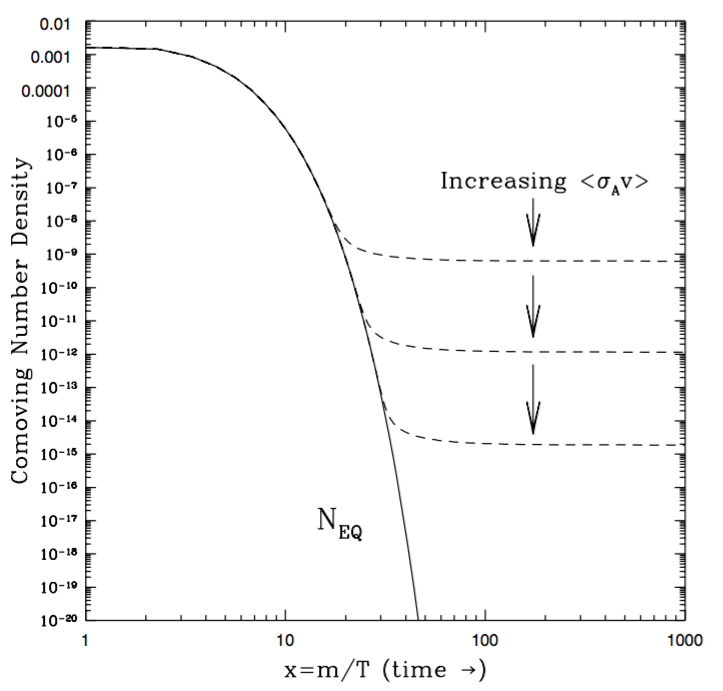
\includegraphics[width=0.7\textwidth]{pictures/FrizzOut}\label{fig2}
%    \caption{{\scriptsize Equilibrium (solid curve) and relic abundance (dashed curve) of WIMP particles. Figure is taken from     arXiv:hep-ph/9506380}}
%    
%\end{figure}

%\end{frame}
% ------------------------------------------------------------------------------------------------

\section{Collider searches for DM}

%\begin{frame}
%\frametitle{Experimental Signature}

%\end{frame}
% ------------------------------------------------------------------------------------------------

\begin{frame}
\frametitle{One-muon  + jet channel}
{\small
The process chows in Figure \ref{TowFerminon}, leads to the signature opposite sign leptons plus missing energy however, 
\begin{itemize}

\item for small $\Delta m(F-S)$ the probability that one or both leptons are not detected in the collider increases. 
\item $p p \to F^+ F^- j $ provides a jet which can be used as a trigger.

\end{itemize}
}
\begin{figure}[!tbp]
\centering
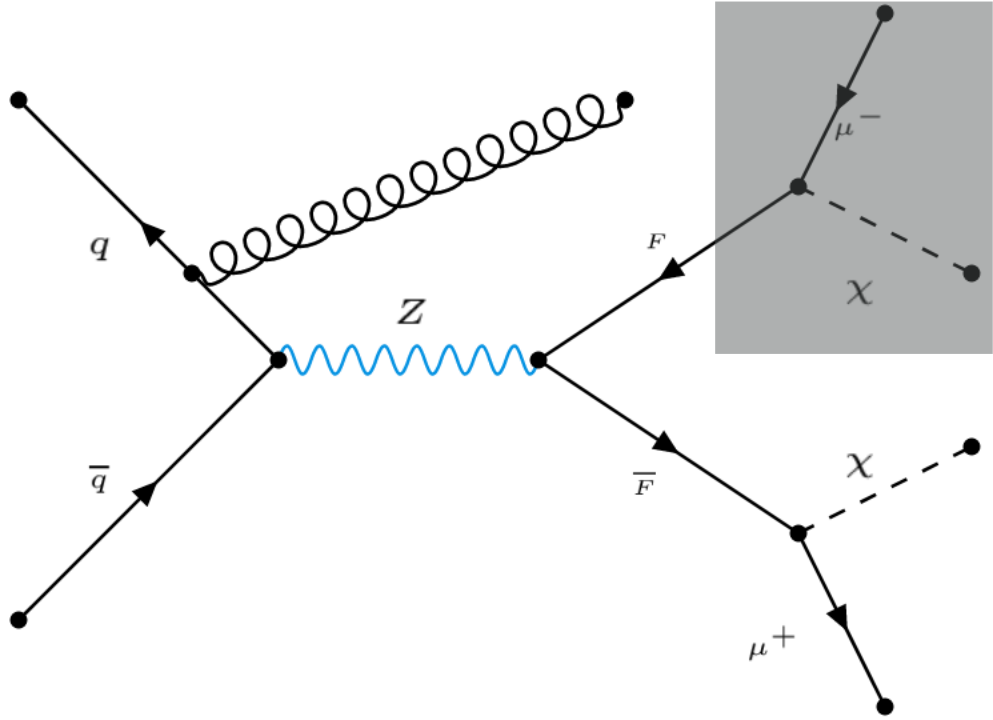
\includegraphics[width=0.45\textwidth]{pictures/DYVLFOneMuon}\label{fig6}
\caption{{\scriptsize Pair-production of vector-like fermions, followed by their decay into a lepton and the DM particle, one missing lepton and a ISR jet }}

\end{figure}

\end{frame}

% ------------------------------------------------------------------------------------------------
\begin{frame}
\frametitle{Parameter Region}

\begin{figure}[!tbp]
\centering
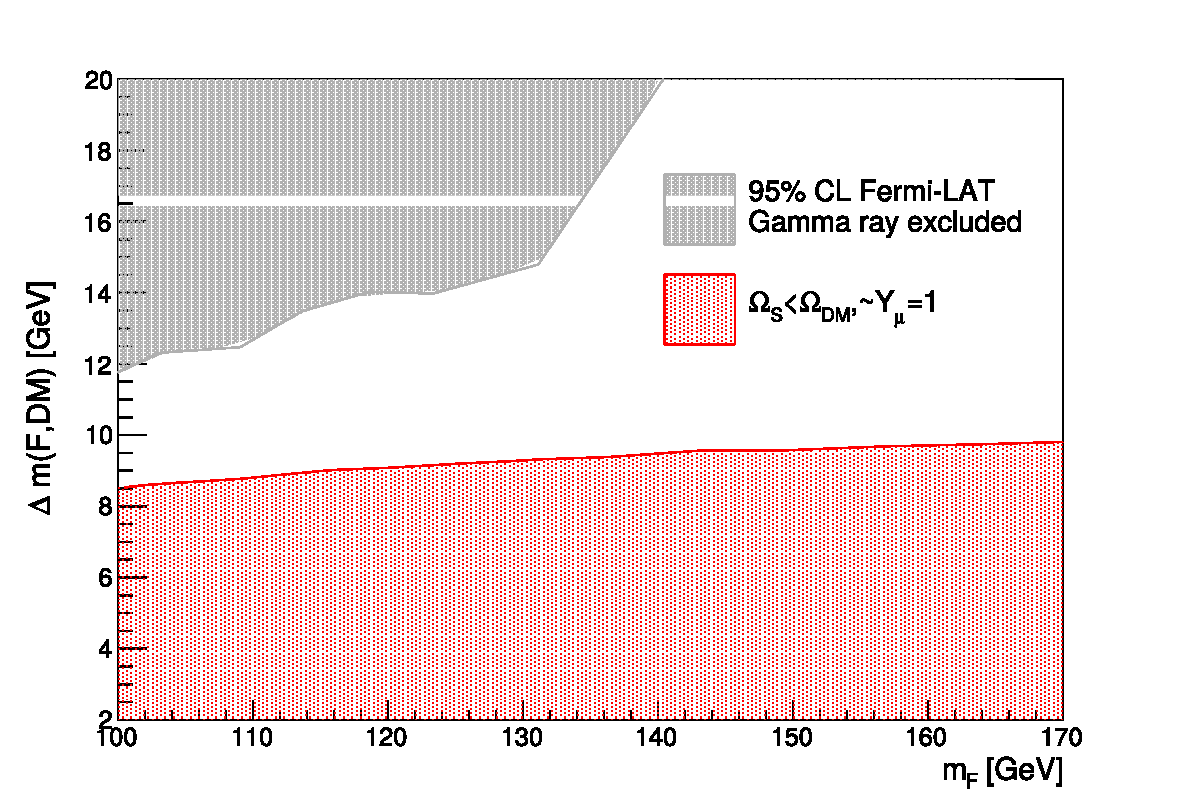
\includegraphics[width=0.85\textwidth]{pictures/LimitPlotsTesis}% while the combined upper region with light and dark magenta are the prospects for Cherenkov Telescope Array.
\caption{{\scriptsize $m_F$ vs $\Delta m$. The gray upper region is excluded by Fermi-LAT and H.E.E.S experiments, while the red area is the where the relic density is not satisfy by the model}}
\label{fig7}
\end{figure}


\end{frame}
% ------------------------------------------------------------------------------------------------
% ------------------------------------------------------------------------------------------------
\begin{frame}
\frametitle{Background}
\begin{justify}
The backgrounds process for this search is the single top, the di-boson $WZ$, and $W+jets $. The last one being the most important with production cross-section three orders larger than the others (see Figure \ref{XSSummary}).

\end{justify}

\begin{figure}[!tbp]
\centering
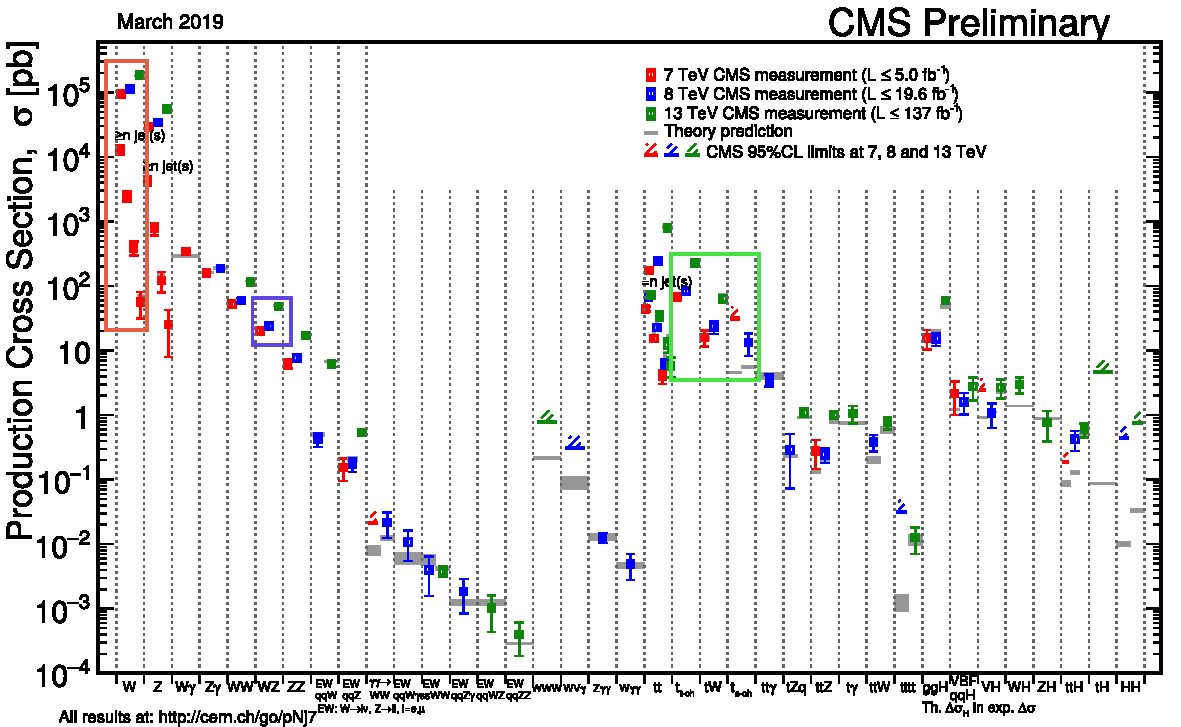
\includegraphics[width=0.7\textwidth]{pictures/CrossSectionSMProcesses}\label{fig8}
\caption{{\scriptsize Summary of the cross section measurements of Standard Model processes [{\tiny https://twiki.cern.ch/twiki/bin/view/CMSPublic/PhysicsResultsCombined}]    }.}
\label{XSSummary}
\end{figure}

\end{frame}
% ------------------------------------------------------------------------------------------------
\begin{frame}
\section{Samples Generation}
\frametitle{Samples Generation}
\begin{justify}
The Monte Carlo(MC) collision samples for the signal and the BackGrounds (BG) were generated using a combination of MadGraph (version 2.5.5 )$^1$ %\cite{Alwall2011} 
for the event generation, Pythia (version 8.233)$^2$ 
for the hadronization and Delphes (version 3.4.1)$^3$  %\cite{deFavereau:2013fsa} 
for the detector effect emulation.
\end{justify}

\begin{spacing}{0.5}
{\tiny
1. \textbf{Alwall, J. et al} T. MadGraph 5: going beyond. J. High Energy Phys. 2011, 128 (2011).

2. \textbf{Sjöstrand, T. et al.} An Introduction to PYTHIA 8.2. Comput. Phys. Commun. 191, 159–177 (2015).

3. \textbf{De Favereau, J. et al}. DELPHES 3, A modular framework for fast simulation of a generic collider experiment. JHEP 02, 57 (2014).
}
\end{spacing}
\end{frame}

% ------------------------------------------------------------------------------------------------

\begin{frame}
\section{Samples Selection}
\frametitle{Selection criteria}
\begin{justify}
The values for the cuts were defined through an optimization process based on both the significance $\mathcal{Z}$ (defined in the \ref{Sig}) and the efficiency of the cut (defined in the \ref{Eff}) of the signal Vs. BG 

\begin{equation}
\mathcal{Z}=\frac{S}{\sqrt{S+B}},\label{Sig}
\end{equation}

where $S$ and $B$ are the yields for Signal and BG. We normalize all MC to $100~\text{fb}^{-1}$ luminosity and the    signal mass point  $m_{F}=145$ GeV vs  $\Delta m=10$ GeV

\begin{equation}
e_{ff}(\chi)=\frac{\chi_{AC}}{\chi_{BC}},\label{Eff}
\end{equation}
were $\chi$ can be signal or BG, and the subscripts $BC$ and $AC$ stands for "Before Cuts" and "After Cuts".

\end{justify}

\end{frame}

% ------------------------------------------------------------------------------------------------
% ------------------------------------------------------------------------------------------------

\begin{frame}
\frametitle{$m_T$ Selection}

\begin{justify}
{\tiny Most signal (bottom-right figure) events are around $50$ GeV, but for all BG the peak of events is more towards $80$ GeV, especially the $W+Jets$. That is why we chose to take a cut of the type \textbf{Less-Than}.}
\end{justify}

\begin{figure}[!h]
\centering
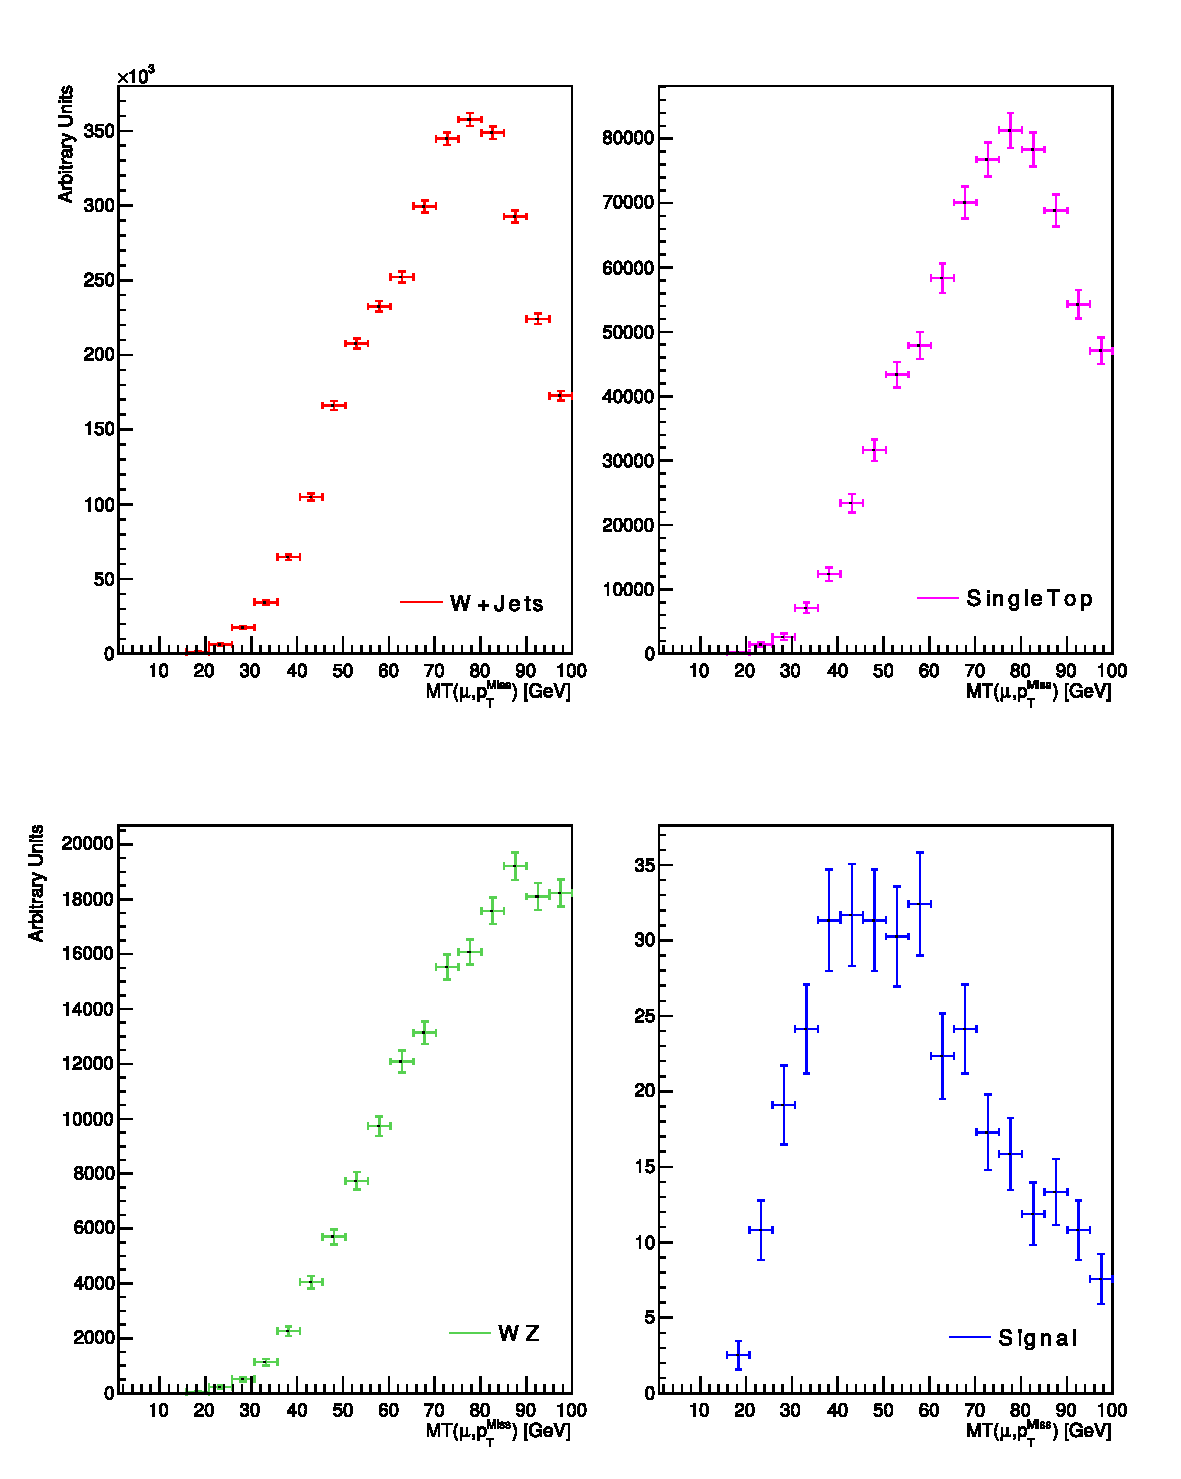
\includegraphics[width=0.75\textwidth, height=0.63\textheight]{pictures/Selection/m_T/All-m_T}
\caption{{\scriptsize $M_T(\mu,p^{miss}_T)$ histograms for the signal and each background sample. The bin-width is 5 GeV. Only the basic selection has been applied.}}
\label{All-m_T}

\end{figure}

\end{frame}

% ------------------------------------------------------------------------------------------------
% ------------------------------------------------------------------------------------------------

\begin{frame}
\frametitle{$m_T$ Selection}
\begin{figure}[!h]

\centering
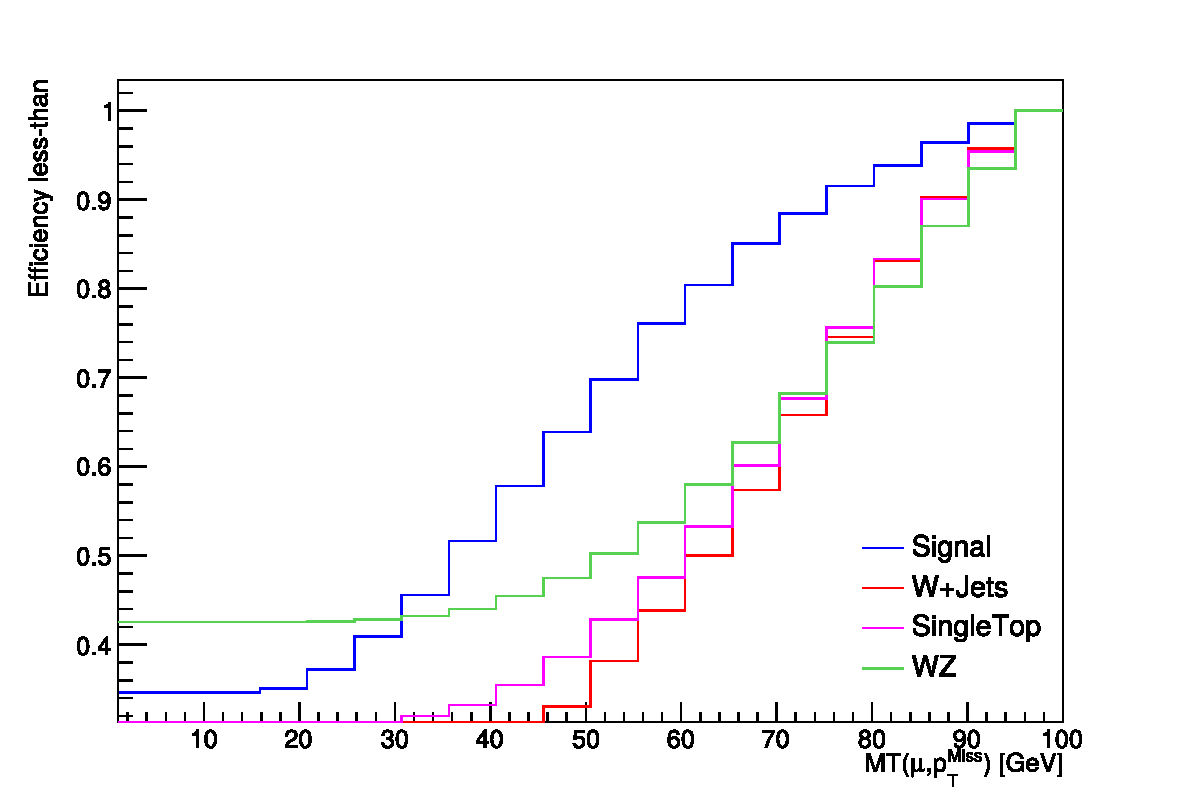
\includegraphics[scale=0.45]{pictures/Selection/m_T/Eff-m_T}
\caption{{\scriptsize $M_T(\mu,p^{miss}_T)$ Efficiency plots for the signal and each background sample. The main BG is less than $1\%$ before $40$ GeV, although the signal is more than $50\%$.}}
\label{Eff-m_T}

\end{figure}


\end{frame}

% ------------------------------------------------------------------------------------------------
% ------------------------------------------------------------------------------------------------

\begin{frame}
\frametitle{$m_T$ Selection}

\begin{figure}[!h]

\centering
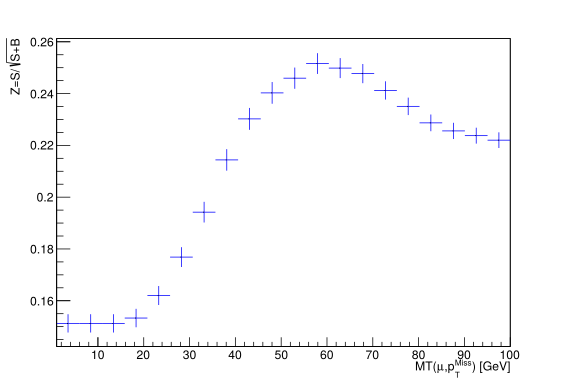
\includegraphics[scale=0.45]{pictures/Selection/m_T/Sig-m_T}
\caption{{\scriptsize Significance of the cut (type less-than) for $m_T(\mu,p_{T}^{Miss})$ . The maximum of $\mathcal{Z}$ is reached for $60$ GeV, but to take out the majority of the $W+jet$ BG events, the cut at $40$ GeV is preferred.}}
\label{Sig-m_T}

\end{figure}


\end{frame}

% ------------------------------------------------------------------------------------------------
% ------------------------------------------------------------------------------------------------


\begin{frame}
\frametitle{$p_T(\mu)$ Selection}

\begin{justify}
{\scriptsize Most signal events are concentrated at low values of $p_T$ as it was expected. It is chosen a less-than cut .}
\end{justify}

\begin{figure}[!h]

\centering
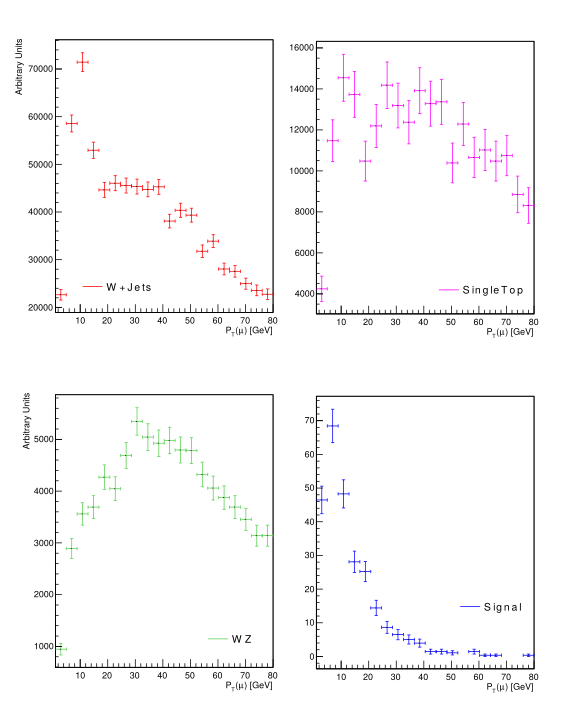
\includegraphics[width=0.7\textwidth, height=0.6\textheight]{pictures/Selection/P_TMu/All-P_TMu}
\caption{{\scriptsize $p_T(\mu)$ histograms for the signal and each background sample. The bin-width is 5 GeV. Besides the basic selection, the cut $M_T<40$ GeV was made.}}
\label{P_TMu}

\end{figure}


\end{frame}

% ------------------------------------------------------------------------------------------------
% ------------------------------------------------------------------------------------------------

\begin{frame}
\frametitle{$p_T(\mu)$ Selection}
\begin{figure}[!h]

\centering
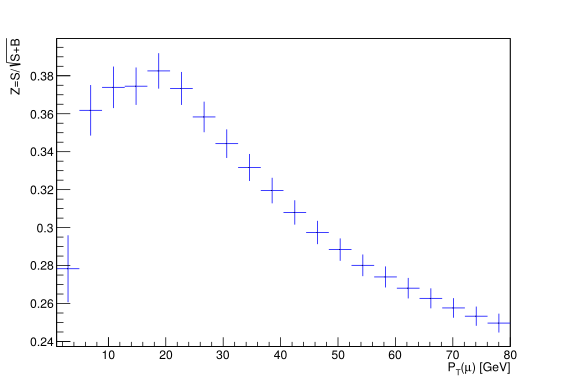
\includegraphics[scale=0.45]{pictures/Selection/P_TMu/Sig-P_TMu}
\caption{{\scriptsize Significance of the cut (type less-than) for $p_T(\mu,)$. The $\mathcal{Z}$ curve reach the maximum at $p_T(\mu,)<20$ GeV and falls fast for higher values.}}
\label{Sig-P_TMu}

\end{figure}


\end{frame}


% ------------------------------------------------------------------------------------------------
% ------------------------------------------------------------------------------------------------

\begin{frame}
\frametitle{$p_T(\mu)$ Selection}
\begin{figure}[!h]

\centering
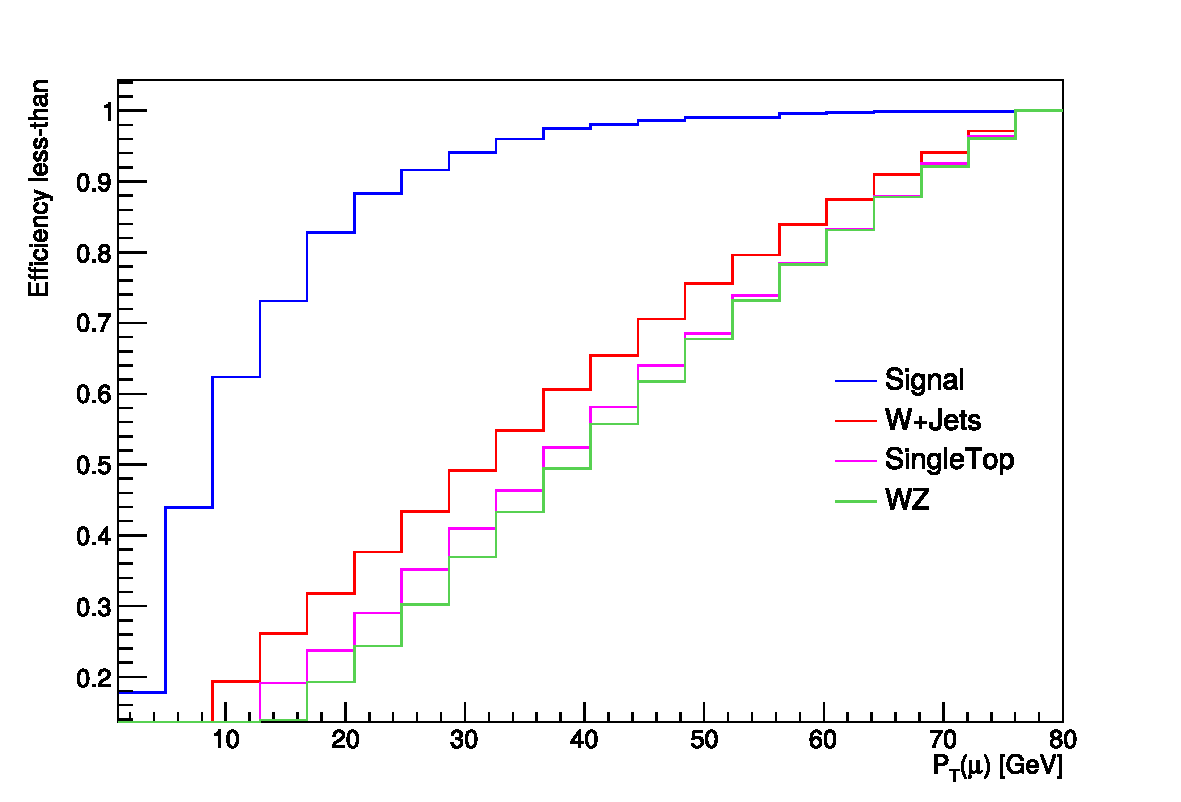
\includegraphics[scale=0.4]{pictures/Selection/P_TMu/Eff-P_TMu}
\caption{{\scriptsize$p_T(\mu)$ efficiency plots for the signal and each background sample. For the cut suggested by Figure \ref{Sig-P_TMu}, the signal reach more than $80\%$ of efficiency, while the main BG is less than $40\%$, confirming the cut based on the significance.}}
\label{Eff-P_TMu}

\end{figure}


\end{frame}

% ------------------------------------------------------------------------------------------------
% ------------------------------------------------------------------------------------------------


\begin{frame}
\frametitle{$N(Jet)$ Selection}
\begin{justify}
{\scriptsize The signal, W+jets, and WZ BG have similar behavior, but to reduce the Single Top events a less-than cut can be used.}
\end{justify}

\begin{figure}[!h]

\centering
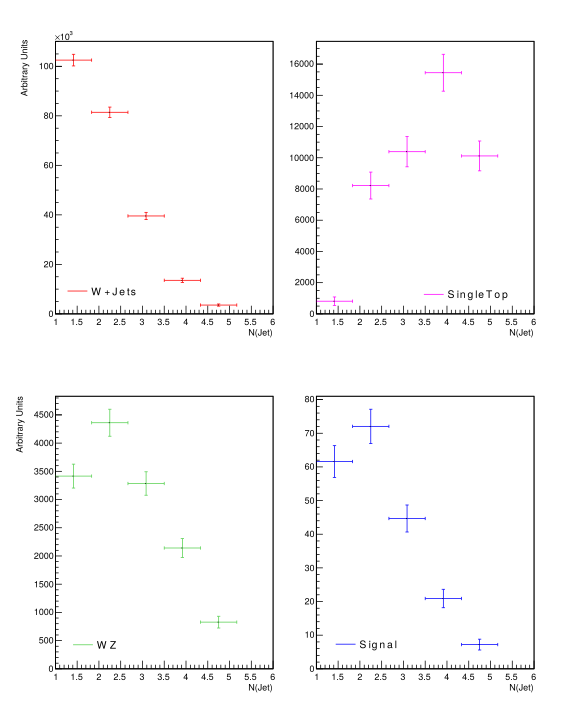
\includegraphics[width=0.75\textwidth, height=0.65\textheight]{pictures/Selection/NJet/All-NJet}
\caption{{\scriptsize $N(Jet)$ histograms. The cuts applied are: the basic selection, $M_T<40$ GeV and $p_T(\mu,)<20$~GeV.}}
\label{All-NJet}

\end{figure}


\end{frame}

% ------------------------------------------------------------------------------------------------
% ------------------------------------------------------------------------------------------------

\begin{frame}
\frametitle{$N(Jet)$ Selection}
\begin{figure}[!h]

\centering
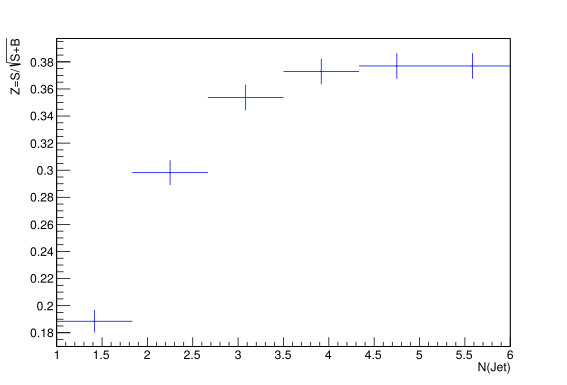
\includegraphics[scale=0.45]{pictures/Selection/NJet/Sig-NJet}
\caption{{\scriptsize The Significance for $N(Jet)$ reach its maximum at $N(Jet)< 4$.}}
\label{Sig-NJet}

\end{figure}


\end{frame}


% ------------------------------------------------------------------------------------------------
% ------------------------------------------------------------------------------------------------

\begin{frame}
\frametitle{$N(Jet)$ Selection}
\begin{figure}[!h]

\centering
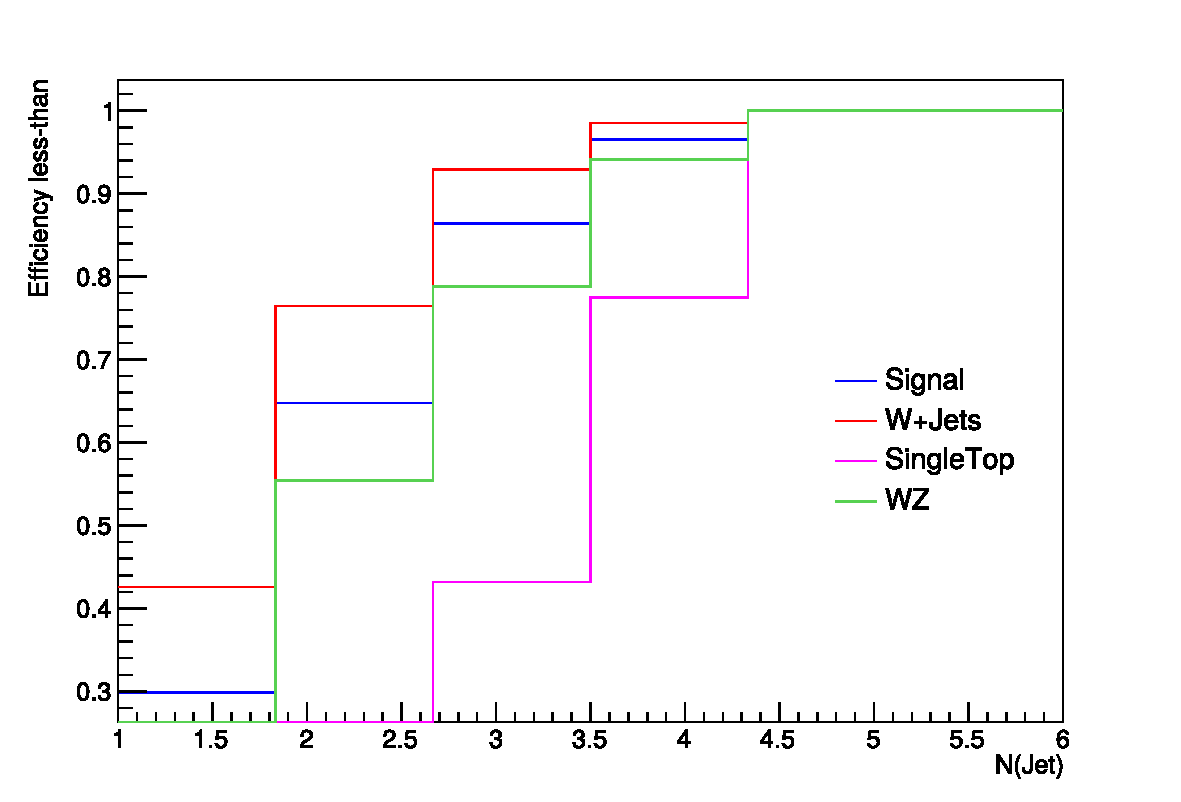
\includegraphics[scale=0.45]{pictures/Selection/NJet/Eff-NJet}
\caption{{\scriptsize The $N(Jet)$ efficiencies. For the signal at  $N(Jet)< 4$ the efficiency is almost $100\%$ while for the main BG is less than $80\%$.}}
\label{Eff-NJet}

\end{figure}


\end{frame}

% ------------------------------------------------------------------------------------------------

% ------------------------------------------------------------------------------------------------


%%\begin{frame}
%%\frametitle{$p_T(Jet)$ Selection}
%%\begin{figure}[!h]

%%    \centering
%    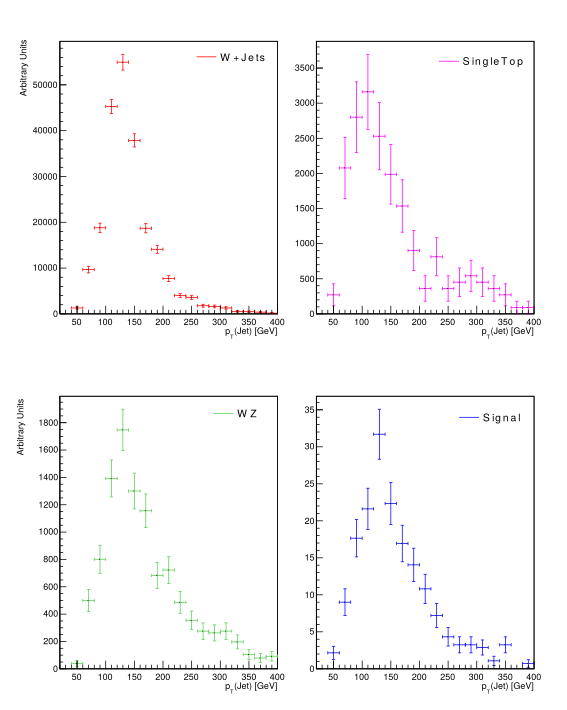
\includegraphics[width=0.9\textwidth, height=0.8\textheight]{pictures/Selection/P_TJet/All-p_TJet}
%    \caption{}
%    \label{All-p_TJet}
%    
%\end{figure}


%\end{frame}

% ------------------------------------------------------------------------------------------------
% ------------------------------------------------------------------------------------------------

%\begin{frame}
%\frametitle{$p_T(Jet)$ Selection}
%\begin{figure}[!h]
%
%\centering
%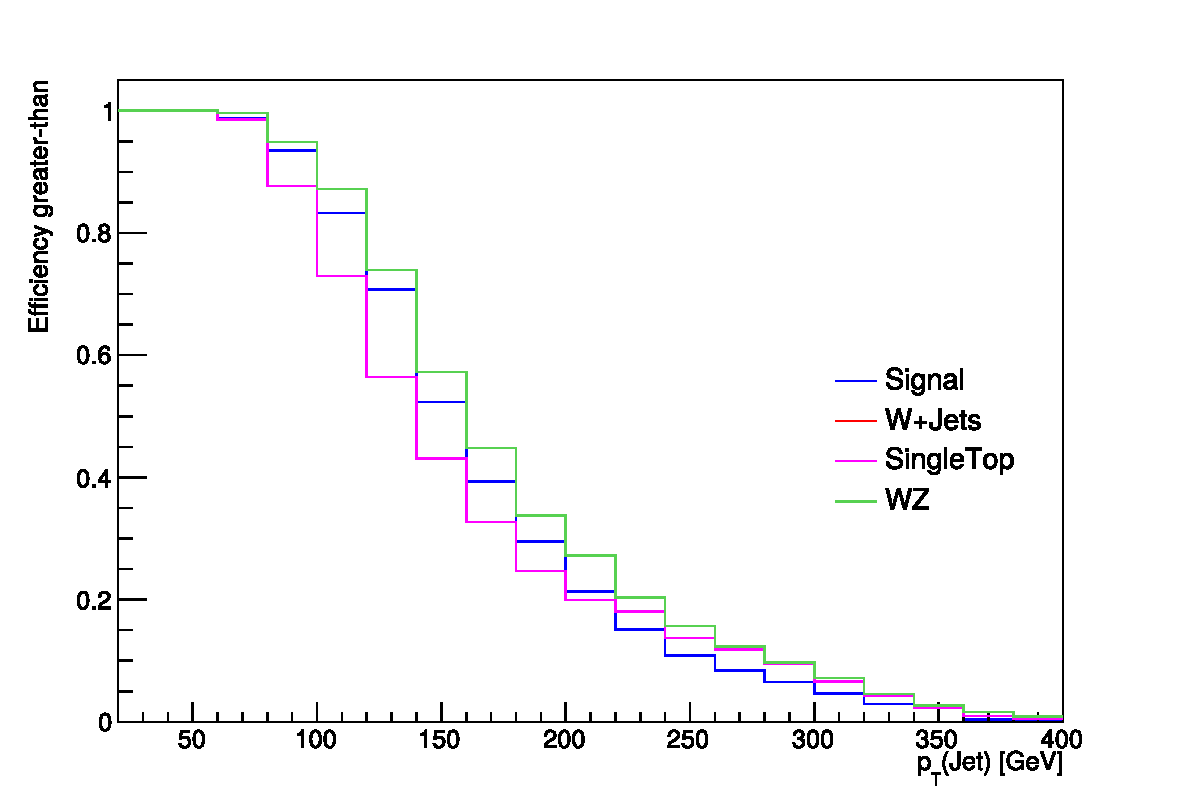
\includegraphics[scale=0.45]{pictures/Selection/P_TJet/Eff-p_TJet}
%\caption{ }
%\label{Eff-p_TJet}

%\end{figure}


%\end{frame}

% ------------------------------------------------------------------------------------------------
% ------------------------------------------------------------------------------------------------

%\begin{frame}
%\frametitle{$p_T(Jet)$ Selection}
%\begin{figure}[!h]

%\centering
%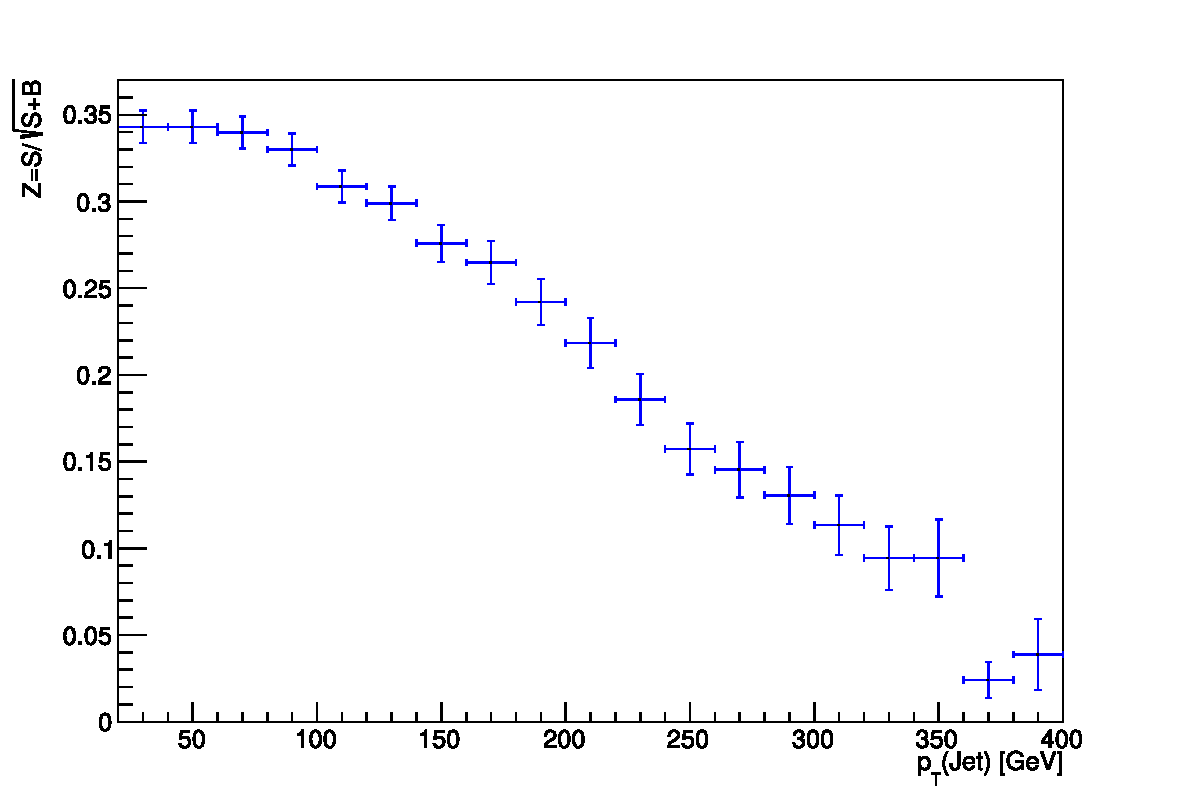
\includegraphics[scale=0.45]{pictures/Selection/P_TJet/Sig-p_TJet}
%\caption{}
%\label{Sig-p_TJet}

%\end{figure}


%\end{frame}


% ------------------------------------------------------------------------------------------------
% ------------------------------------------------------------------------------------------------
\begin{frame}
\frametitle{Selection}
\begin{justify}
In the \textbf{Table \ref{WeightsSamplesTable}} are summarized the cuts made to maximize the significance of the signal, along with the accumulated efficiency after the cut.  

\end{justify}

\begin{table}[]
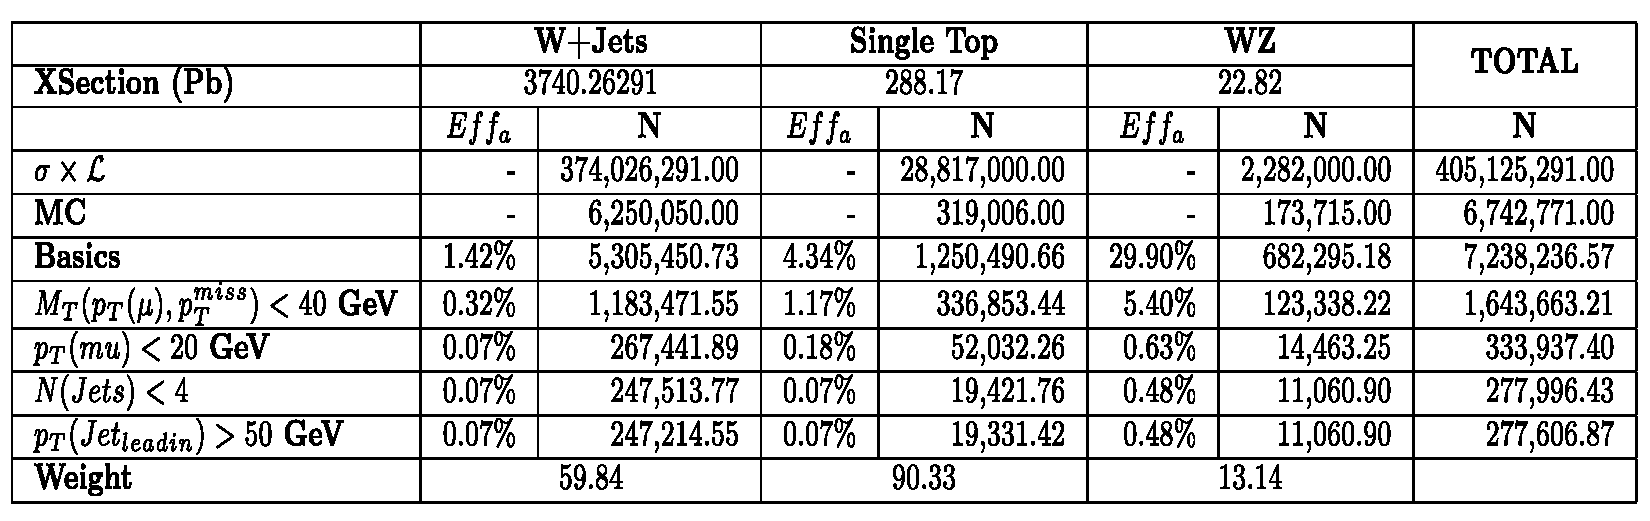
\includegraphics[width=1.0\textwidth]{pictures/Selection/TablaCortes}

\caption{{\scriptsize Weights for the MC samples, based on the expected events, number of MC samples generated for the study, weights for the samples assuming a $100\text{fb}^{-1}$ of luminosity, the number of events, and the accumulated efficiency after each cut.}}
\label{WeightsSamplesTable}
\end{table}

\end{frame}

% ------------------------------------------------------------------------------------------------

% ------------------------------------------------------------------------------------------------
\begin{frame}
\section{Results}
\frametitle{Results}

\begin{figure}
\centering

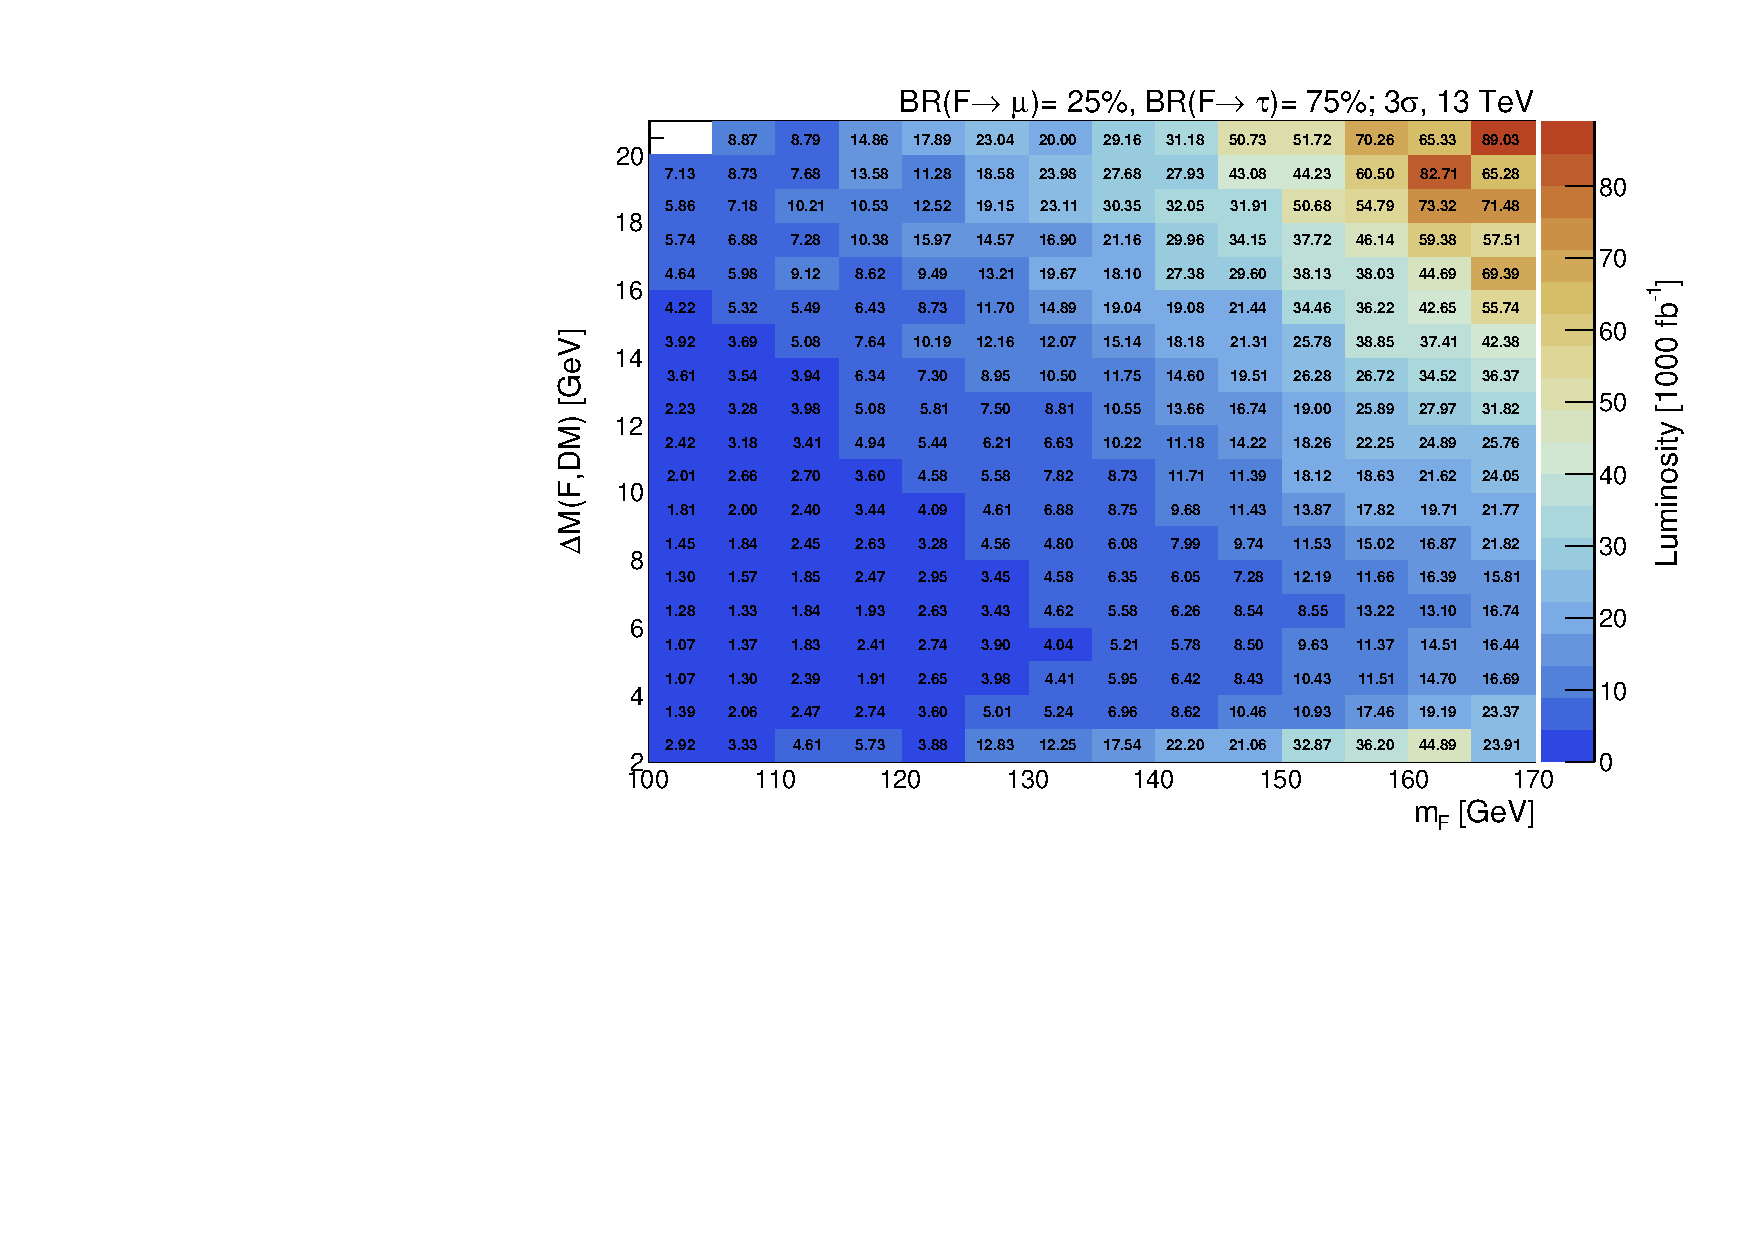
\includegraphics[scale=0.45]{pictures/LumiToExclusionSigma3_BRmu25tau75} 
\caption{3 $\sigma$ reach for $m_{F}$ vs  $\Delta m$ parameter space for various luminosity in $1000\text{fb}^{-1}$. The Yellow line is $3000~\text{fb}^{-1}$}
\label{results}
\end{figure}

\end{frame}

% ------------------------------------------------------------------------------------------------

% ------------------------------------------------------------------------------------------------

\begin{frame}
\frametitle{Exclusion Potential}
\begin{justify}

The exclusion potential of the study is the region of parameters of the model in were at $3000~\text{fb}^{-1}$ the model reach $3\sigma$. part of this region is still unexplored (see \textbf{Figure \ref{fig7}}), the intersection between the regions in \textbf{Figures \ref{fig7}} and \textbf{\ref{results}} is shown in the next slide (Figure \ref{results2}).

The exclusion is carried out assuming that what is going to be observed is the yields due to the SM alone.
\end{justify}
\end{frame}

% ------------------------------------------------------------------------------------------------
% ------------------------------------------------------------------------------------------------
\begin{frame}

\frametitle{Exclusion Potential}

\begin{figure}
\centering

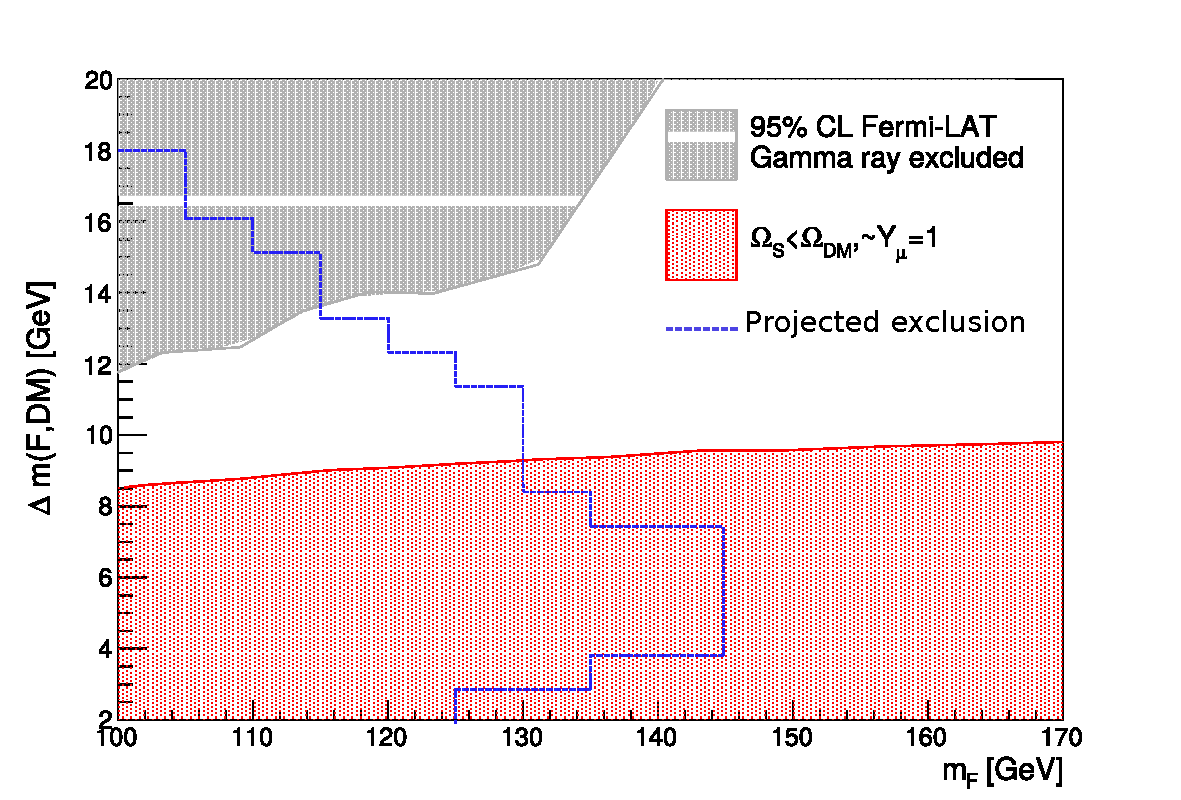
\includegraphics[scale=0.45]{pictures/LimitPlotsTesis_WithData} 
\caption{Exclusion potential of the model. The region left of the yellow line is where the model reach $3\sigma$ of significance at $3000~\text{fb}^{-1}$ of luminosity}
\label{results2}
\end{figure}

\end{frame}

% ------------------------------------------------------------------------------------------------
% ------------------------------------------------------------------------------------------------

\section{Remarks}
\begin{frame}
\frametitle{Remarks}

\begin{exampleblock}{}

\begin{enumerate}

\item Although the model has been analyzed. there is still the region of the parameter space ($\Delta m=m_{F}-m_S\lesssim 50\ \text{GeV}$) with exclusion potential.
\item The full dark matter content may be explained either by freeze-out at higher redshifts or by another dark matter content.
\item  We can obtain exclusion sensitivity over a large region of parameter space has not yet been covered by any other search.
\end{enumerate}

\end{exampleblock}

\end{frame}
% ------------------------------------------------------------------------------------------------



% ------------------------------------------------------------------------------------------------

\ThankYouFrame

% ------------------------------------------------------------------------------------------------

% ------------------------------------------------------------------------------------------------
\section{Backup}

% ------------------------------------------------------------------------------------------------

\begin{frame}
\frametitle{Background Tunig}
{\small To generate the background we use the tunes extract for the data from CMS at the reference [CMS-PAS-GEN-17-001] }

{\scriptsize
	\begin{table}[]
		\begin{tabular}{ll}
			\hline
			\textbf{PYTHIA parameter}                & \textbf{Value} \\\hline
			PDF Set                                  & NNPDF3.1       \\
			$\alpha_S(MZ)$                           & 0.118          \\
			SPACESHOWER:RAPIDITYORDER                & on             \\
			MULTIPARTONINTERACTIONS:ECMREF {[}GeV{]} & 7000           \\
			$\alpha^{ISR}_S$                         & 0.118/NLO      \\
			$\alpha^{FSR}_S$                         & 0.118/NLO      \\
			$\alpha^{MPI}_S$                         & 0.118/NLO      \\
			$\alpha^{ME}_S$                          & 0.118/NLO      \\
			MULTIPARTONINTERACTIONS:PT0REF {[}GeV{]} & 1.41           \\
			MULTIPARTONINTERACTIONS:ECMPOW           & 0.03344        \\
			MULTIPARTONINTERACTIONS:CORERADIUS       & 0.7634         \\
			MULTIPARTONINTERACTIONS:COREFRACTION     & 0.63           \\
			COLORRECONNECTION:RANGE                  & 5.176          \\
			$\chi^2/dof$                             & 1.04           \\\hline
		\end{tabular}
		\caption{Pythia 8 parameter values }
		\label{PythiaTune}
		
	\end{table}
}

\end{frame}


% ------------------------------------------------------------------------------------------------

\begin{frame}
\frametitle{Background Tuning}
After the tunig we use Rivet[] over the analysis [PhysRevD.96.072005] to compare 

\begin{figure}[!h]

\begin{subfigure}[b]{0.44\textwidth}
	\centering
	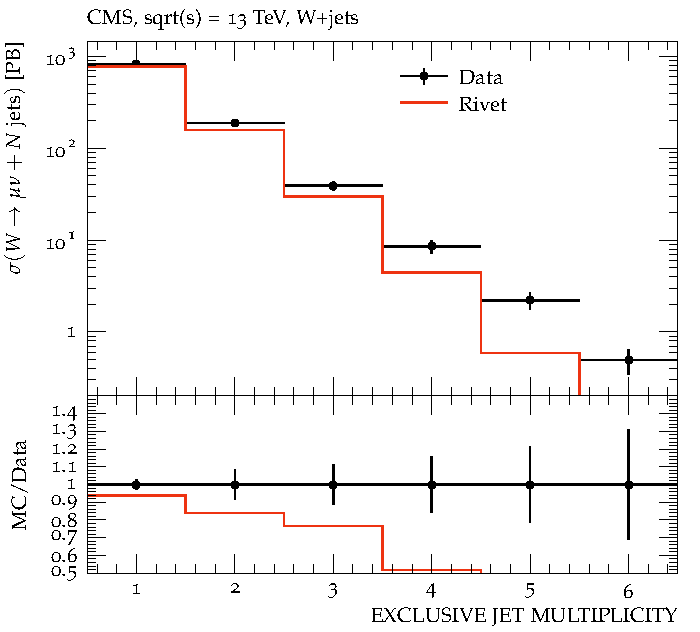
\includegraphics[width=\textwidth]{pictures/MCTunig/EXCLUSIVE_JET_MULTIPLICITY}
	\caption{\label{EXCLUSIVE_JET_MULTIPLICITYTune}}
\end{subfigure}
\begin{subfigure}[b]{0.44\textwidth}
	\centering
	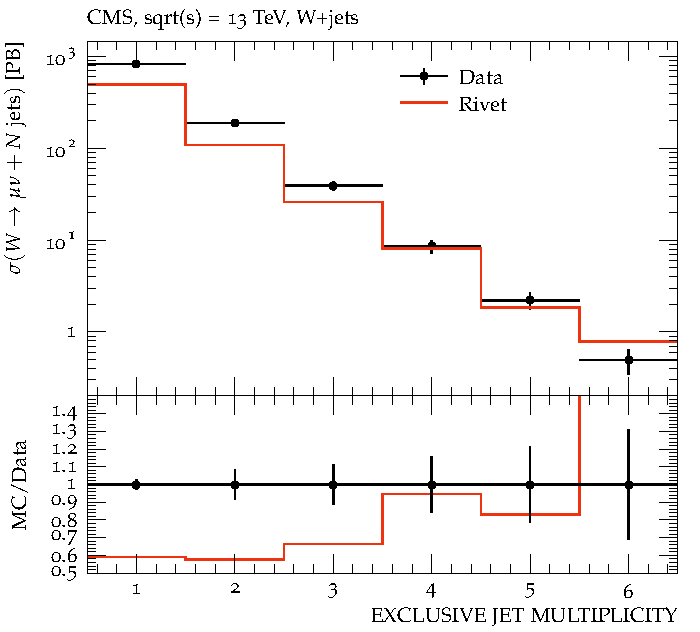
\includegraphics[width=\textwidth]{pictures/MCTunig/EXCLUSIVE_JET_MULTIPLICITY_Nelson}
	\caption{\label{EXCLUSIVE_JET_MULTIPLICITY}}
\end{subfigure}
\caption{ \justifying{ Differential cross section measurement for the exclusive jet multiplicities with tune (\subref{EXCLUSIVE_JET_MULTIPLICITYTune}) and with out tune (\subref{EXCLUSIVE_JET_MULTIPLICITY})} }
\end{figure}


\end{frame}

% ------------------------------------------------------------------------------------------------
% ------------------------------------------------------------------------------------------------

\begin{frame}
\frametitle{Background Tuning}


\begin{figure}[!h]

\begin{subfigure}[b]{0.44\textwidth}
\centering
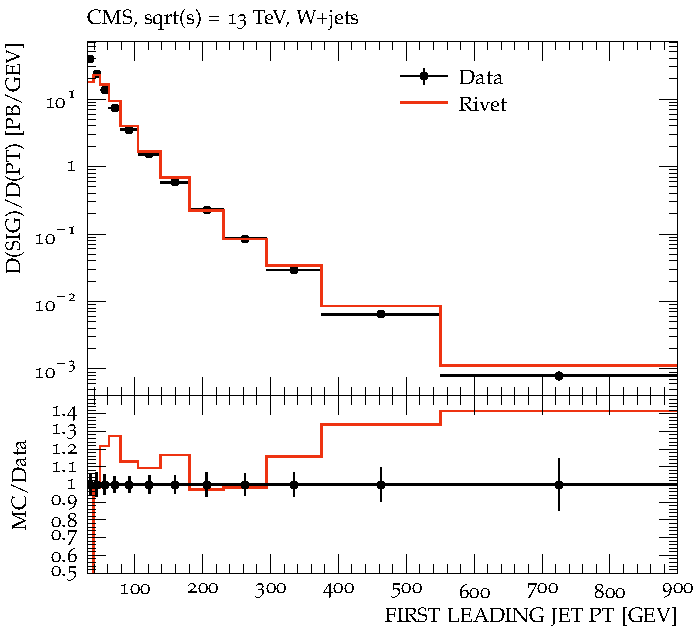
\includegraphics[width=\textwidth]{pictures/MCTunig/FIRST_LEADING_JET_PT}
\caption{\label{FIRST_LEADING_JET_PTTune}}
\end{subfigure}
\begin{subfigure}[b]{0.44\textwidth}
\centering
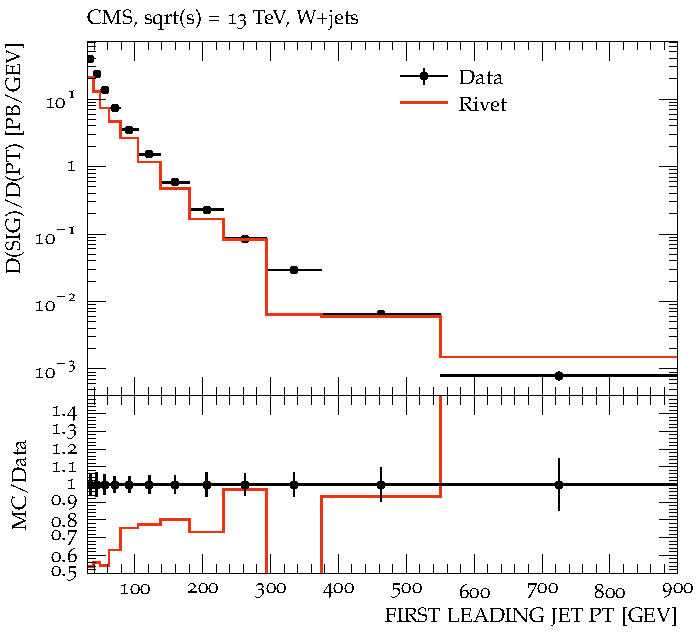
\includegraphics[width=\textwidth]{pictures/MCTunig/FIRST_LEADING_JET_PT_Nelson}
\caption{\label{FIRST_LEADING_JET_PT}}
\end{subfigure}
\caption{ \justifying{ Differential cross section measurement for the exclusive jet multiplicities with tune (\subref{FIRST_LEADING_JET_PTTune}) and with out tune (\subref{FIRST_LEADING_JET_PT})} }
\end{figure}


\end{frame}

% ------------------------------------------------------------------------------------------------
% ------------------------------------------------------------------------------------------------

\begin{frame}
\frametitle{Background Tuning}

\begin{figure}[!h]

\begin{subfigure}[b]{0.44\textwidth}
\centering
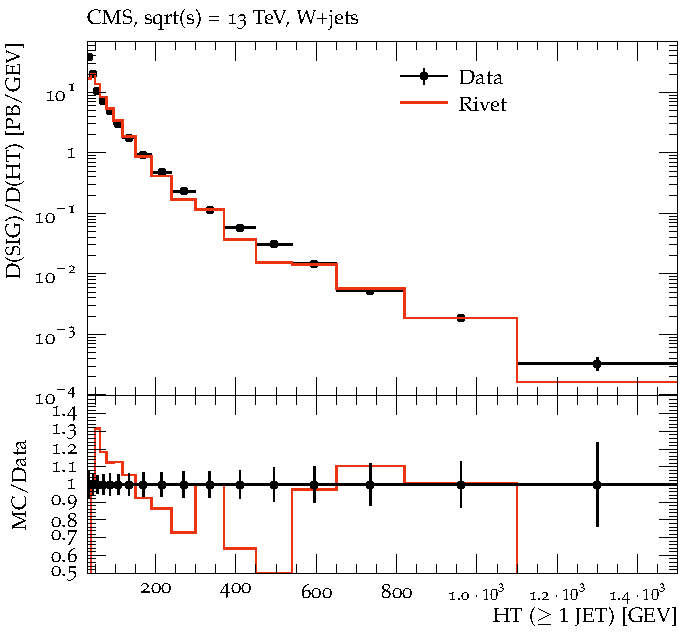
\includegraphics[width=\textwidth]{pictures/MCTunig/HT}
\caption{\label{HTTune}}
\end{subfigure}
\begin{subfigure}[b]{0.44\textwidth}
\centering
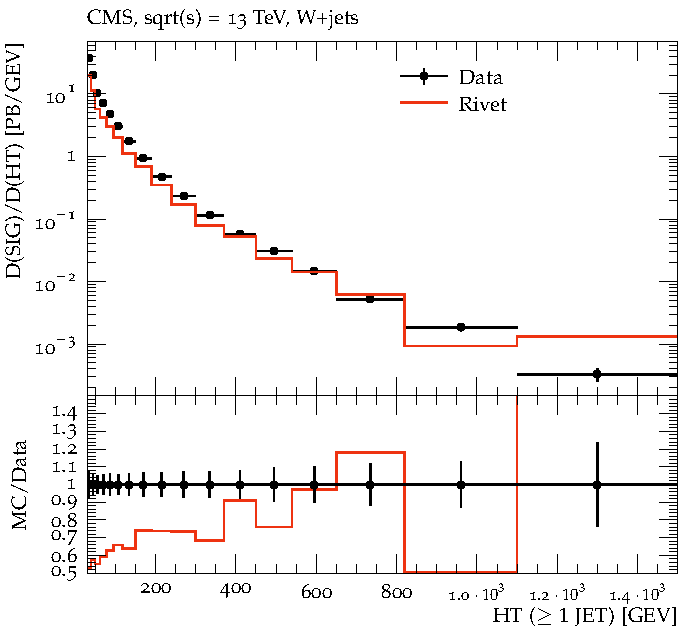
\includegraphics[width=\textwidth]{pictures/MCTunig/HT_Nelson}
\caption{\label{HT}}
\end{subfigure}
\caption{ \justifying{ Differential cross section measurement for the jets HT for at least 1 jet with tune (\subref{HTTune}) and with out tune (\subref{HT})} }
\end{figure}


\end{frame}

% ------------------------------------------------------------------------------------------------

% ------------------------------------------------------------------------------------------------
\begin{frame}
\frametitle{Relation with Fermi LAT}

Gamma-ray from the Galactic center measured these type of models could explain Fermi-LAT Collaboration.

\begin{figure}
\centering
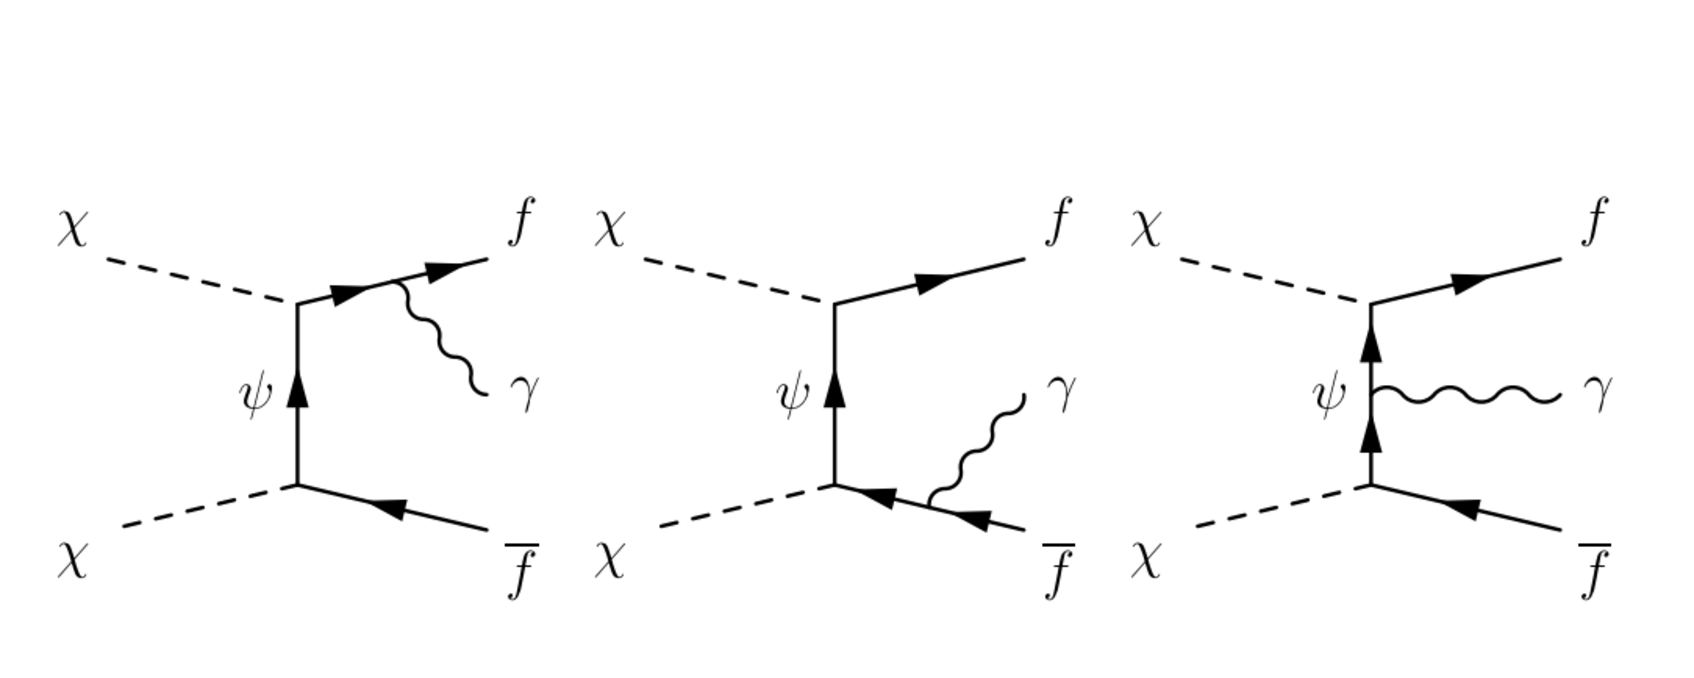
\includegraphics[scale=0.3]{pictures/Bremsstrahlung} 
\caption{Internal Bremsstrahlung processes of (real) scalar DM. From [Toma, T. Phys. Rev. Lett. 111, 91301 (2013)] }
\label{fig:Brem}
\end{figure}

\end{frame}
% ------------------------------------------------------------------------------------------------

% ------------------------------------------------------------------------------------------------
\begin{frame}
\frametitle{Similar Searches}
{\footnotesize
\begin{itemize}
\item Search for top squark pair production in pp collisions at $sqrt(s) = 13$ TeV using single lepton events [J. High Energy Phys. 2017, 19]
\item Search for top squarks decaying via four-body or chargino-mediated modes in single-lepton final states in proton-proton collisions at $sqrt(s) = 13$ TeV [J. High Energy Phys. 2018, 65]

\end{itemize}
}
\begin{figure}
\centering
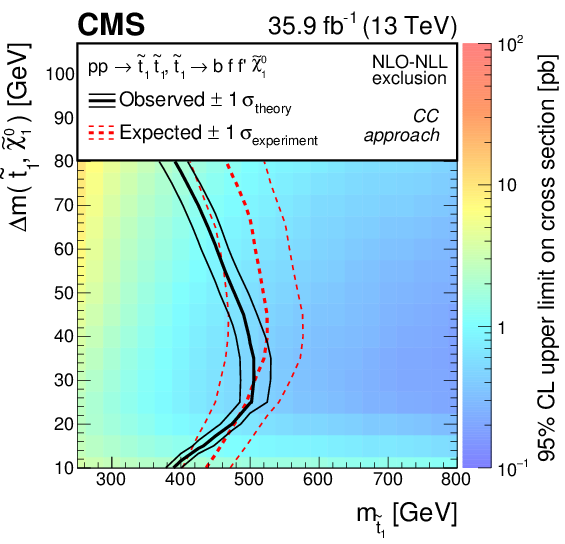
\includegraphics[scale=0.2]{pictures/Figure_007-a} 
\caption{{\scriptsize     Exclusion limit at 95\% for the four-body decay of the top squark as a function of $m(\tilde{t})$ and $\delta m$ } }
\label{04402}
\end{figure}

\end{frame}
% ------------------------------------------------------------------------------------------------



% ------------------------------------------------------------------------------------------------

%\begin{frame}
%\frametitle{M}

%\end{frame}

% ------------------------------------------------------------------------------------------------

% ------------------------------------------------------------------------------------------------

% ------------------------------------------------------------------------------------------------

%\section{Bibliography}
%\begin{frame}{Bibliography}
%\frametitle{Bibliography}

%\bibliographystyle{apalike}
%\bibliography{references}
%\end{frame}

% ------------------------------------------------------------------------------------------------
\end{document}
